% TODO:
%   try to prevent page breaks for shorter listings
%   update website, prominently link to html-thys covered in this paper



% \documentclass[a4paper,UKenglish,cleveref, autoref, thm-restate]{lipics-v2021}
\documentclass[sn-mathphys,Numbered]{sn-jnl}

\usepackage[T1]{fontenc}
\usepackage[utf8]{inputenc}

\usepackage{graphicx}%
\usepackage{multirow}%
\usepackage{amsmath,amssymb,amsfonts}%
\usepackage{amsthm}%
\usepackage{mathrsfs}%
\usepackage[title]{appendix}%
\usepackage{xcolor}%
\usepackage{textcomp}%
\usepackage{manyfoot}%
\usepackage{booktabs}%
\usepackage[boxed]{algorithm}%
\usepackage{algorithmicx}%
\usepackage[noend]{algpseudocode}
\usepackage{listings}%



% \usepackage[T1]{fontenc}
% \usepackage[utf8]{inputenc}
% \usepackage{microtype} % Better typesetting for PDFs -- is enabling this ok?
% \usepackage{balance}


%\usepackage{eufrak} %The eufrak package is redundant if the amsfonts package is used
% \usepackage{mathpartir}
% \DeclareMathAlphabet{\mathpzc}{OT1}{pzc}{m}{it}
% \usepackage[boxed]{algorithm}
% \usepackage{enumerate}
\usepackage{cprotect}

\usepackage{lstautogobble}
\usepackage{tabularx}
\usepackage{ragged2e}  % for '\RaggedRight' macro (allows hyphenation)
\usepackage{caption}
\usepackage[font=scriptsize]{subcaption}
% \usepackage{hyperref}
% \usepackage{float}
% \usepackage{wrapfig}

% \usepackage{multirow}
% \usepackage{siunitx}


\usepackage{tikz}
\usetikzlibrary{positioning,fit,shadows,decorations, arrows, shapes, decorations.markings,decorations.pathmorphing,calc}

\usepackage{pgfplots}


\tikzset{
  -|-/.style={
    to path={
      (\tikztostart) -| ($(\tikztostart)!#1!(\tikztotarget)$) |- (\tikztotarget)
      \tikztonodes
    }
  },
  -|-/.default=0.5,
  |-|/.style={
    to path={
      (\tikztostart) |- ($(\tikztostart)!#1!(\tikztotarget)$) -| (\tikztotarget)
      \tikztonodes
    }
  },
  |-|/.default=0.5,
}

\clubpenalty = 10000
\widowpenalty = 10000
\displaywidowpenalty = 10000

% Not really meant for highlighting isabelle source, but for easily writing latex that looks like
% isabelle
% 
% keyword level 1 - isabelle outer syntax 
% keyword level 2 - isabelle inner syntax programming constructs (if, let, etc)
% keyword level 3 - standard constants (length, mod, etc)
% keyword level 4 - isabelle proof methods


% \newcommand{\lsem}{\ensuremath{\mathopen{[\![}}}
% \newcommand{\rsem}{\ensuremath{\mathclose{]\!]}}}

\lstdefinelanguage{isabelle}{
  morekeywords={theorem,theorems,corollary,lemma,lemmas,locale,begin,end,fixes,assumes,shows,and,class,
    constrains , definition, where, apply, done,unfolding, primrec, fun, using, by, for, uses, file,
    schematic_lemma, concrete_definition, prepare_code_thms, export_code, datatype, type_synonym, typedef, value,
    proof, next, qed, show, have, hence, thus, interpretation, fix, context, sepref_definition,is,export_llvm
 } ,
  morekeywords=[2]{rec, return, bind, foreach, if, then, else, do, let, in, res, spec, fail, assert, while, case, of, 
    check},
%  morekeywords=[3]{length,mod,insert},
%   morekeywords=[4]{simp,auto,intro,elim,rprems,refine_mono,refine_rcg},
  sensitive=True,
  morecomment=[s]{(\*}{\*)},
}


\DeclareTextCommand{\shortunderscore}{T1}{{$\lambda$}}1
  {\\\%}{{$\lambda$}}1
  {\\\$}{{$\mathbin{\,\$\,}$}}1
  {->}{{$\rightarrow$}}1
  {<-}{{$\leftarrow$}}1
  {<.}{{$\langle$}}1
  {.>}{{$\rangle$}}1
  {<=}{{$\le$}}1
  {>=}{{$\ge$}}1
  {<->}{{$\leftrightarrow$}}1
  {-->}{{$\longrightarrow$}}2
  {<-->}{{$\longleftrightarrow$}}1
  {=>}{{$\Rightarrow$}}1
  {==}{{$\equiv$}}2
  {==>}{{$\implies$}}2
  {<=>}{{$\Leftrightarrow$}}1
  {~=}{{$\ne$}}1
  {|}{{$\mid$}}1
  {-`}{{$\rightharpoonup$}}1
  {|`}{{$\restriction$}}1
  {!!}{{$\bigwedge$}}1
  {(}{{$($}}1
  {)}{{$)$}}1
  {\{}{{$\{$}}1
  {\}}{{$\}$}}1
  {[}{{$[$}}1
  {]}{{$]$}}1
  {[|}{{$\llbracket$}}1
  {|]}{{$\rrbracket$}}1
  {\\<lbrakk>}{{$\lsem$}}1
  {\\<rbrakk>}{{$\rsem$}}1
  {|-}{{$\vdash$}}1
  {|=}{{$\models$}}1
  {|->}{{$\mapsto$}}1
  {|_|}{{$\bigsqcup$}}1
  {...}{{$\dots$}}1
  {\\x}{{$\times$}}1
  {_0}{{${}_0$}}1
  {_1}{{${}_1$}}1
  {_2}{{${}_2$}}1
  {_3}{{${}_3$}}1
  {_4}{{${}_4$}}1
  {_5}{{${}_5$}}1
  {_6}{{${}_6$}}1
  {_7}{{${}_7$}}1
  {_8}{{${}_8$}}1
  {_9}{{${}_9$}}1
  {_L}{{${}_L$}}1
  {\\_n}{{${}_n$}}1
  {\\_i}{{${}_i$}}1
  {\\_j}{{${}_j$}}1
  {\\_x}{{${}_x$}}1
  {\\_y}{{${}_y$}}1
  {\\impl}{{${}_\dagger$}}1
  {^*}{{$^*$}}1
  {^k}{{$^k$}}1
  {^d}{{$^d$}}1
  {\\<^sup>*}{{$^*$}}1
  {\\<^sub>*}{{$_*$}}1
  {\\<^sub>A}{{$_A$}}1
  {\\<^sub>r}{{$_r$}}1
  {\\<^sub>a}{{$_a$}}1
  {:_i}{{$:_i$}}1
  {\\<A>}{{$\mathcal{A}$}}1
  {\\<O>}{{\sf o}}1
  {\\<Phi>}{{$\Phi$}}1
  {\\<Psi>}{{$\Psi$}}1
  {\\<sigma>}{{$\sigma$}}1
  {\\<cdot>}{{$\cdot$}}1
  {\\<in>}{{$\in$}}1
  {\\<le>}{{$\le$}}1
  {\\<noteq>}{{$\ne$}}1
  {\\<lambda>}{{$\lambda$}}1
  {\\<longrightarrow>}{{$\longrightarrow$}}1
  {\\<longleftrightarrow>}{{$\longleftrightarrow$}}1
  {\\<Rightarrow>}{{$\Rightarrow$}}1
  {\\<Longrightarrow>}{{$\Longrightarrow$}}1
  {\\<rightarrow>}{{$\rightarrow$}}1
  {\\<leftarrow>}{{$\leftarrow$}}1
  {\\<mapsto>}{{$\mapsto$}}1
  {\\<equiv>}{{$\equiv$}}1
  {\\<and>}{{$\wedge$}}1
  {\\<or>}{{$\vee$}}1
  {\\<And>}{{$\bigwedge$}}1
  {\\<Up>}{{$\Uparrow$}}1
  {\\<Down>}{{$\Downarrow$}}1
  {\\<Union>}{{$\bigcup$}}1
  {\\<up>}{{$\uparrow$}}1
  {\\<down>}{{$\downarrow$}}1
  {\\<times>}{{$\times$}}1
  {\\<forall>}{{$\forall$}}1
  {\\<exists>}{{$\exists$}}1
  {\\<nexists>}{{$\nexists$}}1
  {\\<union>}{{$\cup$}}1
  {\\<inter>}{{$\cap$}}1
  {\\<subset>}{{$\subset$}}1
  {\\<subseteq>}{{$\subseteq$}}1
  {\\<supset>}{{$\supset$}}1
  {\\<supseteq>}{{$\supseteq$}}1
  {\\<alpha>}{{$\alpha$}}1
  {\\<beta>}{{$\beta$}}1
  {\\<gamma>}{{$\gamma$}}1
  {\\alpha}{{$\alpha$}}1
  {\\beta}{{$\beta$}}1
  {\\gamma}{{$\gamma$}}1
  {\\<Gamma>}{{$\Gamma$}}1
  {\\<langle>}{{$\langle$}}1
  {\\<rangle>}{{$\rangle$}}1
  {\\<not>}{{$\neg$}}1
  {\\<box>}{{$\oblong$}}1
  {\\<bot>}{{$\bot$}}1
  {\\<top>}{{$\top$}}1
  {\\<notin>}{{$\notin$}}1
  {\\<guillemotright>}{{$\gg$}}1
  {\\in}{$\in$}1
  {\\and}{$\wedge$}1
  {\\or}{$\vee$}1
  {\\Phi}{{$\Phi$}}1
  {\\Psi}{{$\Psi$}}1
  {\\le}{{$\le$}}1
  {\\Up}{{$\Uparrow$}}1
  {\\Down}{{$\Down$}}1
  {>>}{{$\gg$}}1
  {>>=}{{${\gg}{=}$}}1
  {<*lex*>}{{$\times_{\sf lex}$}}1
  {\\<open>}{{\rm\guilsinglleft}}1
  {\\<close>}{{\rm\guilsinglright}}1
}

% \newcommand{\is}{\lstinline[language=isabelle,basicstyle=\normalsize\ttfamily\slshape]}
\newcommand{\is}{\lstinline[language=isabelle]}
\newcommand{\q}[1]{\mbox{\guilsinglleft{#1}\hspace{-.0pt}\guilsinglright}}
% \newcommand{\isai}[1]{\q{\lstinline[language=isabelle,basicstyle=\normalsize\ttfamily\slshape]{#1}}}
\cMakeRobust\q

\lstset{captionpos=b}
\lstset{numberbychapter=false}
\lstset{autogobble}


\newcolumntype{Y}{>{\RaggedRight\arraybackslash}X} % Multiline column, automatic width




  \newcommand{\false}{\textrm{false}}
  \newcommand{\true}{\textrm{true}}

\theoremstyle{thmstyleone}%
\newtheorem{theorem}{Theorem}%  meant for continuous numbers
%%\newtheorem{theorem}{Theorem}[section]% meant for sectionwise numbers
%% optional argument [theorem] produces theorem numbering sequence instead of independent numbers for Proposition
\newtheorem{proposition}[theorem]{Proposition}%
%%\newtheorem{proposition}{Proposition}% to get separate numbers for theorem and proposition etc.

\theoremstyle{definition}%
\newtheorem{example}{Example}%
\newtheorem{remark}{Remark}%

\theoremstyle{thmstylethree}%
\newtheorem{definition}{Definition}%

\raggedbottom

\begin{document}


\title[Refinement of Parallel Algorithms down to LLVM]{Refinement of Parallel Algorithms down to LLVM}
\subtitle{applied to practically efficient parallel sorting}

\author*[1]{\fnm{Peter} \sur{Lammich}}\email{p.lammich@utwente.nl}
\affil*[1]{\orgdiv{Faculty of Electrical Engineering, Mathematics and Computer Science} \orgname{University of Twente} \orgaddress{\city{Enschede} \country{Netherlands}}}


\abstract{
  We present a stepwise refinement approach to develop
  verified parallel algorithms, down to efficient LLVM code.
  The resulting algorithms' performance is competitive with their
  counterparts implemented in C++.
%
  Our approach is backwards compatible with the Isabelle Refinement Framework,
  such that existing sequential formalizations can easily be adapted
  or re-used.
%
  As case study, we verify a parallel quicksort algorithm that is
  competitive to unverified state-of-the-art algorithms.
}

\keywords{Isabelle,Concurrent Separation Logic,Parallel Sorting,LLVM}


\maketitle


\section{Introduction}
% Modern hardware has become faster by getting more parallel, while the
% sequential execution speed has not significantly increased in the last years.
% To keep up with this development, and fully utilize the capabilities of modern hardware,
% parallel algorithms are required.
%
% However, parallel algorithms come with new subtle classes of errors, like race conditions,
% which are particularly hard to find by testing. Thus, formal methods that can guarantee
% absence of all errors, including the hard-to-find ones, become even more important for
% parallel algorithms.

We present a stepwise refinement approach to develop
verified and efficient parallel algorithms. Our method can verify total correctness down to LLVM intermediate code.
The resulting verified implementations are competitive with state-of-the-art
unverified implementations. Our approach is backwards compatible to
the Isabelle Refinement Framework (IRF)~\cite{La19-llvm}, a powerful tool to verify efficient sequential software,
such as model checkers~\cite{ELNN13,BrLa18,WiLa18}, SAT solvers~\cite{La17_CADE,La17_SAT,FBL18},
or graph algorithms~\cite{La14,LaSe16,LaSe19}.
This paper adds parallel execution to the IRF's toolbox, without invalidating the existing formalizations,
which can now be used as sequential building blocks for parallel algorithms, or be modified to add
parallelization.

As a case study, we verify total correctness of a parallel quicksort algorithm,
re-using an existing verification of state-of-the-art sequential sorting algorithms~\cite{La20}.
Our verified parallel sorting algorithm is competitive to state-of-the-art parallel sorting algorithms
from GNU's C++ standard library and the Boost C++ Libraries.

This paper is an extended version of our ITP 2022 paper~\cite{La22}.
The main new contribution is a verified parallel partitioning algorithm,
which significantly improves the efficiency and scalability of our sorting algorithm from~\cite{La22}.
To this end, we added a description of the interval list data structure (Section~\ref{sec:mod_ds})
and the \is{with_idxs} combinator (Section~\ref{sec:array_split}), which are required by the parallel partitioner.
The parallel partitioning algorithm itself is described in Section~\ref{sec:ppar}, and Section~\ref{sec:benchmark}
contains updated and more extensive benchmarks.


% The main idea is to add a parallel combinator to an existing
% sequential LLVM semantics, by extending the thread semantics to record memory accesses, and
% check these for data-race freedom upon joining the parallel threads.
% Based on this idea, we extend the existing Isabelle Refinement Framework~\cite{La19-llvm}
% to support parallel algorithms. The resulting framework is largely backwards compatible to
% the original one, such that we could easily port existing algorithms and data structures,
% and use them as building blocks for parallel algorithms.


% The contributions of this paper are as follows:
% \begin{itemize}
%   \item the (up to our knowledge) first verification method for parallel LLVM programs.
%
%   \item a stepwise refinement approach to verify total correctness of parallel programs.
%
%   \item the first verified implementation of a parallel sorting algorithm.
% \end{itemize}

The formalization is available at \href{https://www21.in.tum.de/~lammich/isabelle_llvm_par/}{www21.in.tum.de/$\sim$lammich/isabelle\_llvm\_par}.


\subsection{Overview}\label{sec:intro_overview}
This paper is based on the Isabelle Refinement Framework, a continuing effort
to verify efficient implementations of complex algorithms, using stepwise refinement techniques~\cite{LaLo10,LaTu12,La13,La15,La19-llvm,HaLa21}.
Figure~\ref{fig:IRF-overview} displays the components of the Isabelle Refinement Framework.
%
\begin{figure}
  \definecolor{colA}{RGB}{11, 97,164}
  \definecolor{colB}{RGB}{204,246,  0}
  \definecolor{colC}{RGB}{166,  0,166}
  \definecolor{colD}{RGB}{255,146,  0}
  \definecolor{colTCB}{RGB}{255, 0, 0}


  \center
  \begin{tikzpicture}[node distance=.01\textwidth,outer sep=0pt,
  basicLayer/.style={
    draw=black,
    rounded corners,
    text width=.9\textwidth,
    font={\sffamily\bfseries\color{black}},
    align=center,
    minimum height=.03\textheight,
%    text height=12pt,
%    text depth=9pt
    },
  layerA/.style={basicLayer,fill=colA!30},
  layerB/.style={basicLayer,fill=colB!30},
  layerC/.style={basicLayer,fill=colC!30},
  layerD/.style={basicLayer,fill=colD!30},
  layerDD/.style={basicLayer,fill=colD!40,text width=.2\textwidth},
  layerTCB/.style={basicLayer,fill=colTCB!30,text width=.2\textwidth},
  layerTCBB/.style={basicLayer,fill=colTCB!40,text width=.2\textwidth},
  ]

  \node[layerA] (AlgDS) {Algorithms and Data Structures};

  \node[layerB, below=of AlgDS.south west, anchor=north west, text width=.437\textwidth] (ne) {NE-Monad};
  \node[layerA, right=of ne.north east, anchor=north west, text width=.437\textwidth, minimum height=.067\textheight] (llDS) {Low-Level Algorithms \\and Data Structures};

  \node[layerB, below=of ne.south west, anchor=north west, text width=.437\textwidth] (sepref) {Sepref};

  \node[layerC, below=of sepref.south west, anchor=north west] (sepl) {Program Logic and VCG};
  \node[layerD, below=of sepl.south west, anchor=north west, minimum height=.13\textheight] (sembox) {};

  \node[layerTCB, below left=of sembox.north east, minimum height=.12\textheight, text width=.537\textwidth] (tcbbox) {};


  \node[right=of sembox.west,text width=.2\textwidth,font={\sffamily\bfseries\color{black}}] {Back\\ End};

  \node[above left=of tcbbox.south east,font={\sffamily\bfseries\color{black}}] {Trusted Code Base};

%   \node[layerD, right=of sembox.west] (preproc) {Preprocessor};
%   \node[layerD, right=1cm of preproc] (instr) {Instructions};
%   \node[layerD, right=1cm of instr] (codegen) {Code Generator};

  \node[layerTCBB, below left=of tcbbox.north east] (codegen) {Code Generator};
  \node[layerTCBB, left=1cm of codegen] (instr) {Instructions};
  \node[layerDD, left=1cm of instr] (preproc) {Preprocessor};


  \node[layerTCBB, below=of instr] (mmodel) {Memory Model};
  \node[layerTCBB, below=of mmodel] (mmonad) {SE-Monad};

  \draw[->] (preproc) -- (instr);
  \draw[->] (instr) -- (codegen);


  \end{tikzpicture}

  \caption{Components of the IRF, with focus on the back end.}\label{fig:IRF-overview}
\end{figure}
%
The back end layer handles the translation from Isabelle/HOL to the actual target language.
The instructions of the target language are shallowly embedded into Isabelle/HOL, using
a state-error (SE) monad. An instruction with undefined behaviour,
or behaviour outside our supported fragment, raises an error.
The state of the monad is the memory, represented via a memory model.
The code generator translates the instructions to actual code.
These components form the trusted code base, while all the remaining components of the
Isabelle Refinement Framework generate proofs. In the back-end, the preprocessor transforms
expressions to the syntactically restricted format required by the code generator,
proving semantic equality of the original and transformed expression.
While there exist back ends for purely functional code~\cite{LaTu12,La13},
and sequential imperative code~\cite{La15,La19-llvm}, this paper describes a back end
for parallel imperative LLVM code (Section~\ref{sec:parsem}).

On top of the back-end, we formalize a concurrent separation logic~\cite{OH04} and implement a verification condition generator (VCG), cf.\ Section~\ref{sec:seplogic}.

At the level of the program logic and VCG, our framework can be used to verify simple low-level algorithms and data structures,
like dynamic arrays and linked lists. More complex developments typically use a stepwise refinement approach,
starting at purely functional programs modelled in a nondeterminism-error (NE) monad~\cite{LaTu12}.
A semi-automatic refinement procedure (Sepref~\cite{La15,La19-llvm}) translates from the purely functional
code to imperative code, refining abstract functional data types to concrete imperative ones.
In Section~\ref{sec:refine_parallel}, we describe our extensions to support refinement to parallel executions,
and a fine-grained tracking of pointer equalities, required to parallelize computations that work on
disjoint parts of the same array.

Using our approach, complex algorithms and data structures can be developed and
refined to optimized efficient code. The stepwise refinement ensures a separation of concerns
between high-level algorithmic ideas and low-level optimizations. We have already used this approach to
verify a wide range of practically efficient sequential algorithms~\cite{ELNN13,BrLa18,WiLa18,La17_CADE,La17_SAT,FBL18,La14,LaSe16,LaSe19,La20}.
In Section~\ref{sec:parsort}, we use our extended techniques to verify a parallel sorting algorithm,
with competitive performance wrt.\ unverified state-of-the-art algorithms.

Section~\ref{sec:concl} concludes the paper and discusses related and future work.


%
% While the ne-monad and associated tooling has largely stayed the same since it's first version~\cite{LaTu12},
% the Sepref tool has been continuously adapted and improved with each new back end that was added.
% Again, our work is based on the Sepref tool for LLVM without time~\cite{La19-llvm}.
%
%
% While the Imperative HOL versions of the IRF are based on a separation logic formalization
% by Lammich and Meis~\cite{LaMe12}, the LLVM versions are based on a more general framework by Klein et al.~\cite{KKB12,KKB12_afp}.
%
% While this reasoning infrastructure can already be used to verify simple low-level algorithms and data structures,
% more complex developments are typically refined from a purely functional,
% monadic representation of nondeterministic programs (ne-monad), originally introduced in~\cite{LaTu12}.
% A typical development will do multiple refinement steps inside the ne-monad, and then use a
% semi-automatic tool (Sepref) to refine from the ne-monad into the back end semantics.
% While the ne-monad and associated tooling has largely stayed the same since it's first version~\cite{LaTu12},
% the Sepref tool has been continuously adapted and improved with each new back end that was added.
% Again, our work is based on the Sepref tool for LLVM without time~\cite{La19-llvm}.
%
% We have also implemented parallelism for the Imperative HOL back end.
% This was done as a feasibility study, and uses the exactly same ideas and
% techniques as described in this paper for the more efficient LLVM back end.
% While a description of this initial implementation would not add any new
% ideas to this paper, it might still be useful in the context of older developments,
% that have not yet been ported to the LLVM back end.
%
% The rest of this paper is roughly organized along the structure of the Isabelle Refinement Framework:
% We first describe our parallel LLVM semantics (Section~\ref{sec:parsem}) and separation logic~\ref{sec:seplogic}.
% Then, we describe our changes to the refinement infrastructure (Section~\ref{sec:refine_parallel}).
% Section~\ref{sec:parsort} describes our parallel sorting algorithm case study and benchmark results,
% and Section~\ref{sec:concl} concludes the paper and discusses related and future work.
%

%
%
%
% Contributions
%   shallow embedding of parallel semantics
%
%   technical: formalization of parallel separation logic. TOTAL CORRECTNESS.
%   integration of parallel call into refinement framework. backwards compatible (re-use of seq).
%
%   technical: automatic refinement with concrete-identity tracking
%
%   formalization of simple parallel quicksort, using state-of-the-art sequential sort as subroutine
%
%   sample partitioning scheme, template instantiation by preprocessor

\subsection{Notation}
Formal statements in this paper correspond to theorems proved in our Isabelle/HOL formalization,
though sometimes simplified to improve the clarity of the presentation.

We mainly use Isabelle/HOL notation, with some shortcuts and adaptations for presentation in a paper.
In this section, we give examples of the more unusual notations: for implication, we always write \is{==>},
e.g., \is{\<forall>x. x\:<\:4 ==> x\:<=\:4} (in Isabelle, one must use \is{-->} here). Free variables are
universally quantified at the top-level.

Type variables are \is{'a, 'b, ...} and function types are written curried as \is{'a => 'b => 'c}.
Types can be annotated to any term, e.g., \is{(x::nat)\:<\:4 ==> x\:<=\:3}.
Function application is written as \is{f x y}, and function update is \is{f(x:=y)}.
For definitions, we use \is{==}, e.g., \is{f x == x+1}.

Algebraic datatypes are written as \is{'a option == Some (the: 'a) | None}. This also defines the selector function \is{the :: 'a option => 'a}.
Values of the tuple type \is{'a_1 \x ... \x 'a$_n$} are written as \is{(a_1,...,a$_n$)}. Lists have type \is{'a list},
and we write \is{[]} for the empty list, \is{x#xs} for the list with head \is{x} and tail \is{xs}, and \is{xs_1@\:xs_2} for list concatenation.
We also use the list notation \is{[1,2,3]}. The length of list \is{xs} is \is{|xs|}.

The empty set is \is${} :: 'a set$. The set \is${l..<h}$ contains all elements between $l$ inclusive and $h$ exclusive, and the set \is${l..}$ contains all elements greater than or equal to $l$.
Disjoint union is written as \is{$\dot\cup$}. We only write \is{$\dot\cup$} if it is clear from the context where the disjointness constraint belongs to.
Otherwise, we will explicitly write, e.g., \is$ s = s_1 \union s_2  &  s_1 \inter s_2 = {}$. The cardinality of a finite set \is{s} is \is{|s|}.

Lambda abstraction is written as \is{\<lambda>x. x+1}. When clear from the context, we omit the \is{\<lambda>}, e.g. \is{spec x. x\:>\:42}.
We also use Haskell-like sections for infix operators, e.g. \is{(+1)} for \is{\<lambda>x. x+1}.
We also use underscores to indicate the parameter positions, e.g., \is${_..<_}$ for \is$\<lambda>l h. {l..<h}$.



\section{A Back End for LLVM with Parallel Execution}\label{sec:parsem}
  We formalize a semantics for parallel execution, shallowly embedded into Isabelle/HOL.
  As for the existing sequential back ends~\cite{La15,La19-llvm}, the shallow embedding is key
  to the flexibility and feasibility of the approach.
  The main idea is to make an execution report its accessed memory,
  and use this information to raise an error when joining executions that
  would have exhibited a data race. We use this to model an instruction that
  calls two functions in parallel, and waits until both have returned.

  \subsection{State-Nondeterminism-Error Monad with Access Reports}\label{sec:monad}
  We define the underlying monad in two steps. We start with a nondeterminism-error monad,
  and then lift it to a state monad and add access reports.
  Defining a nondeterminism-error monad is straightforward in Isabelle/HOL:
  \begin{lstlisting}
    'a neM == spec ("'a => bool") | fail
    return x == spec (%r. r=x)
    bind fail f == fail
    bind (spec P) f == if ?x. P x & f x = fail then fail
                            else spec (%r. ?x Q. P x & f x = spec Q & Q r)
  \end{lstlisting}
  A program either fails, or yields a possible set of results (\is{spec P}), described by its characteristic function \is{P}.
  The \is{return} operation yields exactly one result, and \is{bind} combines all possible results,
  failing if there is a possibility to fail. We use the notation \is{x<-m; f x} for \is{bind m (\<lambda>x. f x)},
  and \is{m_1; m_2} for \is{bind m_1 (\<lambda>_. m_2)}.

  Now assume that we have a state (memory) type \is{\mu}, and an access report type \is{\rho}, which forms a monoid (\is{0,+}).
  With this, we define our state-nondeterminism-error monad with access reports, just called \is{M} for brevity:
  \begin{lstlisting}
    'x M == \mu => ('x \x \rho \x \mu) neM
    return$_M$ x \mu == return$_{ne}$ (x,0,\mu)
    bind$_M$ m f \mu == (x_1,r_1,\mu) <- m \mu; (x_2,r_2,\mu) <- f x_1 \mu; return$_{ne}$ (x_2,r_1+r_2,\mu)
  \end{lstlisting}
  Here, \is{return} does not change the state, and reports no accesses (\is$0$),
  and \is{bind} sequentially composes the executions, threading through the state $\mu$ and adding up the access reports \is$r_1$ and \is$r_2$. Note that we use the names \is$r :: \rho$ for reports, \is$\mu :: \mu$ for memory, and \is$m :: _ M$ for monads.

  Typically, the access report will contain read and written addresses, such that data races can be detected.
  Moreover, if parallel executions can allocate memory, we must detect those
  executions where the memory manager allocated the same block in both parallel strands.
  As we assume a thread safe memory manager, those \emph{infeasible} executions can safely be ignored.
  Let \is{feasible :: \rho => \rho => bool} and \is{norace :: \rho => \rho => bool} be symmetric predicates,
  and let \is{combine :: (\rho \x \mu) => (\rho \x \mu) => (\rho \x \mu) } be a commutative operator to
  combine two pairs of access reports and states. Then, we define a parallel composition operator for \is{M}:
  \begin{lstlisting}
    (m_1 || m_2) \mu ==
      (x_1,r_1,\mu_1) <- m_1 \mu; (x_2,r_2,\mu_2) <- m_2 \mu;  --"\rightcomment{execute both strands}"
      assume feasible \rho_1 \rho_2;  --"\rightcomment{ignore infeasible combinations}"
      assert norace \rho_1 \rho_2; --"\rightcomment{fail on data race}"
      return$_{ne}$ ((x_1,x_2), combine (\rho_1,\mu_1) (\rho_2,\mu_2))  --"\rightcomment{combine results}"

    assume P == if P then return () else spec (%_. False)
    assert P == if P then return () else fail
  \end{lstlisting}
  Here, we use \is{assume} to ignore infeasible executions, and \is{assert} to fail on data races.
  Note that, if one parallel strand fails, and the other parallel strand has no possible
  results (\is{spec (\<lambda>_. False)}), the behaviour of the parallel composition is not clear.
  For this reason, we fix an invariant \is{invar$_M$ :: (\mu => ('x \x \rho \x \mu) neM) => bool},
  which implies that every non-failing execution has at least one possible result.
  We define the actual type \is{M} as the subtype satisfying \is{invar$_M$}.
  Thus, we have to prove that every combinator and instruction of our semantics
  preserves the invariant, which is an important sanity check.
  As additional sanity check, we prove symmetry of parallel composition:
  \begin{lstlisting}
    m_1 || m_2 = mswap (m_2 || m_1)     $\text{where}$    mswap m == (x_1,x_2)<-m; return (x_2,x_1)
  \end{lstlisting}
%   where \is|mswap m = (x_1,x_2)<-m; return (x_2,x_1)| swaps the result tuple.

  \subsection{Memory Model}
  Our memory model supports blocks of values, where values can be integers, structures, or pointers into a block:
  \begin{lstlisting}
    bidx == nat
    addr == ADDR bidx nat
    ptr == PTR_NULL   |   PTR_ADDR (the_addr: addr)
    val == LL_INT lint   |   LL_STRUCT val list   |   LL_PTR ptr

    block == FRESH   |   FREED   |   is_alloc: ALLOC (vals: "val list")
    typedef memory == { \mu :: bidx => block. finite {b. \mu b ~= FRESH} }
  \end{lstlisting}
  A block is either fresh, freed, or allocated, and a memory is a mapping from block indexes (\is{bidx}) to blocks,
  such that only finitely many blocks are not fresh. Every block's state transitions from fresh to
  allocated to freed. This avoids ever reusing the same block, and thus allows us to semantically detect use after free errors.
  Every program execution can only allocate finitely many blocks,
  such that we will never run out of fresh blocks\footnote{If the actual system does run out of memory, we will terminate the program in a defined way.}.
  An allocated block contains an array of values, modelled as a list. Thus, an address \is$ADDR bi i$ consists of a block index \is$bi$, and an index \is{i} into the array.

  To access and modify memory, we define the functions \is{valid}, \is{get}, and \is{put}:
  \begin{lstlisting}
    valid \mu (ADDR b i) == is_alloc (\mu b) & i < |vals (\mu b)|
    get \mu (ADDR b i) == vals (\mu b) ! i
    put \mu (ADDR b i) x == \mu(b := ALLOC ((vals (\mu b))[i:=x]))
  \end{lstlisting}
  where \is{|xs|} is the length of list \is{xs}, \is{xs!i} returns the \is$i$th element of list \is$xs$,
  and \is{xs[i:=x]} replaces the \is$i$th element of \is{xs} by \is{x}.

  Note that our LLVM semantics does not support conversion of pointers to integers, nor comparison
  or difference of pointers to different blocks. This way, a program cannot see the internal representation of a pointer,
  and we can choose a simple abstract representation, while being
  faithful wrt.\ any actual memory manager implementation.

  \subsection{Access Reports}
  We now fix the state of the M-monad to be memory, and the access reports to be tuples \is{(r,w,a,f)} of
  read and written addresses, as well as sets of allocated and freed blocks:
  \begin{lstlisting}
    acc == addr set \x addr set \x bidx set \x bidx set
    0 == ( {},{},{},{} )
    (r_1,w_1,a_1,f_1) + (r_2,w_2,a_2,f_2) == ( r_1 \union r_2, w_1 \union w_2, a_1 \union a_2, f_1 \union f_2 )
  \end{lstlisting}

  Two parallel executions are feasible if they did not allocate the same block. They have a data race
  if one execution accesses addresses or blocks modified by the other:
  \begin{lstlisting}
    feasible (r_1,w_1,a_1,f_1) (r_2,w_2,a_2,f_2) == a_1 \inter a_2 = {}

    norace (r_1,w_1,a_1,f_1) (r_2,w_2,a_2,f_2) ==
      let m_1 = w_1 \<union> { ADDR b i. b \<in> a_1 \<union> f_1 } in
      let m_2 = w_2 \<union> { ADDR b i. b \<in> a_2 \<union> f_2 } in
        (r_1 \<union> m_1) \<inter> m_2 = {}   &   m_1 \<inter> (r_2 \<union> m_2) = {}
  \end{lstlisting}
  The combine function joins the access reports and memories,
  preferring allocated over fresh, and freed over allocated memory. When joining two allocated blocks, the written addresses
  from the access report are used to join the blocks. We skip the rather technical definition of combine, and just state the
  relevant properties: Let \is{\rho_1=(r_1,w_1,a_1,f_1)} and \is{\rho_2=(r_2,w_2,a_2,f_2)} be feasible and race free access reports,
  and \is{\mu_1, \mu_2} be memories that have evolved from a common memory \is{\mu}, consistently with
  the access reports \is{\rho_1, \rho_2}. Let \is{(\rho',\mu') = combine (\rho_1,\mu_1) (\rho_2,\mu_2)}. Then
  \begin{lstlisting}
    (1)  \mu' b = FRESH <--> \mu b = FRESH \and b ~: a_1 \union a_2
    (2)  is_alloc (\mu' b) <--> (is_alloc (\mu b) \or b \<in> a_1 \union a_2) \and b ~: f_1 \union f_2
    (3)  \mu' b = FREED <--> \mu b = FREED \or b \in f_1 \union f_2
  \end{lstlisting}
  Moreover, for all addresses \is{addr = ADDR b i} with \is{valid \mu' addr}:
  \begin{lstlisting}
    (4)  addr \in w_1 \or b \in a_1 ==> get \mu' addr = get \mu_1 addr
    (5)  addr \in w_2 \or b \in a_2 ==> get \mu' addr = get \mu_2 addr
    (6)  addr ~: w_1\:\<union>\:w_2 & b ~: a_1\:\<union>\:a_2 ==> get \mu' addr = get \mu addr
  \end{lstlisting}
  The properties (1)--(3) define the state of blocks in the combined memory:
  a fresh block in \is{\mu'} was fresh already in \is{\mu}, and has not been allocated (1);
  an allocated block was already allocated or has been allocated, but has not been freed (2); and a freed block was already freed, or has been freed (3).
  The properties (4)--(6) define the content: addresses written or allocated in the first or second execution get their content from \is{\mu_1} (4) or \is{\mu_2} (5) respectively.
  Addresses not written nor allocated at all keep their original content (6).

  \subsection{The Interface of the M-Monad}
  The invariant for \is{M} states that blocks transition only from fresh to allocated to free,
  allocated blocks never change their size, and the access report matches the observable state change (\is{consistent}).
  It also states, that for each finite set of blocks $B$, there is an execution that does not allocate blocks from $B$.
  The latter is required to show that we always find feasible parallel executions:
  \begin{lstlisting}
    invar$_M$ c == \<forall>\mu P. c \mu = spec P ==>
      (\<forall>x \rho \mu'. P (x,\rho,\mu') ==> consistent \mu \rho \mu')
    & (\<forall>B. finite B ==> (\<exists>x \rho \mu'. P (x,\rho,\mu') & \rho.a \inter B = {} ))
  \end{lstlisting}

  To define functions in the M-monad, we have to show that they satisfy this invariant.
  For \is{return} and \is{bind}, this is straightforward. The proof for the parallel operator is slightly more involved,
  using the properties of \is{combine}, and the invariant for the operands to obtain a feasible parallel execution.

  Moreover, the M monad provides the memory management functions \is{Mmalloc}, \is{Mfree}, \is{Mload}, \is{Mstore}, and \is{Mvalid_addr}.
  The latter function checks if a given address is valid, and is used to check if pointer arithmetic can be performed
  on that address. Currently, it behaves like loading from that address, in particular it does not support pointers
  one past the end of an allocated block. We leave integration of such pointers to future work.

  \begin{example}[{Memory Allocation}]
    To define memory allocation in \is{M}, we first define the allocation function in the underlying nondeterminism-error monad:
    \begin{lstlisting}
    malloc vs \mu ==
      b <- spec b. is_FRESH \mu b;
      return (b, ({},{},{b},{}), \mu(b:=ALLOC vs))
    \end{lstlisting}
    This function selects an arbitrary fresh block \is$b$, and initializes it with the given list \is$vs$ of values.
    It returns the allocated block, an access report for the allocation, and the updated memory.

    We then show that \is{malloc} satisfies the invariant of M: we correctly report the allocated block.
    Moreover, we can select any fresh block. As our memory model guarantees an infinite supply of fresh blocks,
    any finite set of blocks can be avoided.
    \begin{lstlisting}
      invarM_malloc: invarM (malloc vs)
    \end{lstlisting}

    Finally, we define the corresponding function in the M monad, using Isabelle's lifting and transfer package~\cite{HuKu13}:
    \begin{lstlisting}
      lift_definition Mmalloc :: val list => M is malloc by (rule invarM_malloc)
    \end{lstlisting}
    The other memory management functions are defined analogously.
  \end{example}

  \subsection{LLVM Instructions}
  Based on the M-monad, we define shallowly embedded LLVM instructions. For most instructions,
  this is analogous to the sequential case~\cite{La19-llvm}.
  Additionally, we define an instruction for a parallel function call:
  \begin{lstlisting}
    llc_par f g a b == f a || g b
  \end{lstlisting}
  The code generator only accepts this, if \is{f} and \is{g} are constants (i.e., function names).
  It then generates some type-casting boilerplate, and a call to an external
  \is{parallel} function, which we implement using the Threading Building Blocks~\cite{TBB} library:
  \begin{lstlisting}[language=C++, basicstyle=\ttfamily]
  void parallel(void (*f1)(void*), void (*f2)(void*), void *x1, void *x2) {
    tbb::parallel_invoke([=]{f1(x1);}, [=]{f2(x2);}); }
  \end{lstlisting}
  I.e., the two functions \is{f1(x1)} and \is{f2(x2)} are called in parallel. The generated boilerplate code sets up \is{x1} and \is{x2} to point to both, the actual arguments and space for the results.










%
%
%
%
%
%
%
%
%
%
%   \subsection{Executions}\label{sec:parsem:execs}
%   To model executions, we use a state-nondeterminism-error monad, where each execution reports the memory that it has accessed.
%   This information is used to make a parallel execution fail in case of data races.
%   We start with a standard nondeterminism-error (ne) monad, where an execution either fails, or returns a set of possible results, specified by its characteristic function.
%   \begin{lstlisting}
%     'a neM == spec ("'a => bool") | fail
%     return x == spec (%r. r=x)
%     bind fail f == fail
%     bind (spec P) f == if ?x. P x & f x = fail then fail
%                       else spec (%r. ?x Q. P x & f x = spec Q & Q r)
%   \end{lstlisting}
%   We use the shortcut notation \is{x<-m; f x} for \is|bind m (\<lambda>x. f x)|.
%
%   In the \is{ne}-monad, we can define the functions for memory management. We define functions for memory allocation,
%   freeing, loading, and storing. In addition to returning a result and a new memory, these functions also return
%   information which memory was accessed, i.e., the read and written addresses, as well as the allocated and freed blocks:
%   \begin{lstlisting}
%     macc == { r: addr set; w: addr set; a: nat set; f: nat set }
%   \end{lstlisting}
%   Memory accesses form a commutative monoid where \is{0} means no accesses, and \is{(+)} joins the accesses.
%   \begin{lstlisting}
%     0 == { r={},w={},a={},f={} }
%     {r_1,w_1,a_1,f_1} + {r_2,w_2,a_2,f_2} == { r=r_1\union r_2, w=w_1\union w_2, a=a_1\union a_2, f=f_1\union f_2 }
%   \end{lstlisting}
%
%   We display the definitions of memory allocation and storing. Freeing and loading are defined analogously:
%   \begin{lstlisting}
%     alloc :: val list => memory => (nat \x macc \x memory)
%     alloc vs \mu ==
%       b <- spec b. \mu b = FRESH;  --"\rightcomment{Select some fresh block}"
%       return (b, macc (r={},w={},a={b},f={}), \mu(b:=ALLOC vs))
%
%     store :: addr => val => memory => (unit \x macc \x memory)
%     store addr v \mu ==
%       assert valid \mu addr;
%       return ((), macc (r={},w={addr},a={},f={}), put \mu addr v)
%
%     assert True == return ()     assert False == fail
%   \end{lstlisting}
%   The \is{alloc} function nondeterministically selects a fresh block of memory, and initializes it
%   with the given list \is{vs} of values. Additionally, it reports an allocation access of the allocated block.
%   The \is{store} function checks if the given address is valid. Then, it updates the memory and reports a write access.
%   Here, \is{assert} fails if the argument is false.
%
%   Next, we lift these definitions to a monad of type \is{'a M = memory => ('a \x macc \x memory)}.
%   The return function does not modify the state and reports no memory accesses, and bind sequentially composes
%   the state change, and joins the reported memory accesses:
%   \begin{lstlisting}
%     return$_M$ x \mu == return$_{ne}$ (x,0,\mu)
%
%     bind$_M$ m f \mu == (x,acc_1,\mu) <- m \mu; (r,acc_2,\mu) <- f x \mu; return$_{ne}$ (r,acc_1+acc_2,\mu)
%   \end{lstlisting}
%   note that we use subscripts ${}_{M}$ and ${}_{ne}$ to disambiguate the monad operations when not clear from context.
%
%   Moreover, we define parallel execution:
%   \begin{lstlisting}
%     (m_1 || m_2) \mu ==
%       (x_1,acc_1,\mu_1) <- m_1 \mu; (x_2,acc_2,\mu_2) <- m_2 \mu;  --"\rightcomment{execute both strands}"
%       assume acc_1.a \inter acc_2.a = {};  --"\rightcomment{Filter out impossible combinations}"
%       assert norace acc_1 acc_2; --"\rightcomment{fail on data race}"
%       return$_{ne}$ ((x_1,x_2),acc_1+acc_2, combine \mu_1 acc_2 \mu_2 )  --"\rightcomment{Combine results}"
%
%     assume P == if P then return () else spec (%_. False)
%   \end{lstlisting}
%   That is, we execute both programs from the initial memory \is{\mu}.
%   Then, we filter out impossible executions, i.e., where the memory manager allocated the
%   same block in both branches. For the remaining executions, we fail if there is a data race, i.e.,
%   if the accessed addresses and blocks of one strand interfere with the modified addresses and blocks
%   of the other strand:
%   \begin{lstlisting}
%     intf_norace acc_1 acc_2 ==
%       let m_1 = acc_1.w \<union> { ADDR b i. b \<in> acc_1.a \<union> acc_1.f } in
%       let m_2 = acc_2.w \<union> { ADDR b i. b \<in> acc_2.a \<union> acc_2.f } in
%       (acc_1.r \<union> m_1) \<inter> m_2 = {}  &   m_1 \<inter> (acc_2.r \<union> m_2) = {}
%   \end{lstlisting}
%   Finally, we combine the memories from the two executions, using the reported memory accesses.
%   The \is{combine \mu_1 acc_2 \mu_2} function combines the memories, amending \is{mu_1}
%   with values from \is{mu_2} at blocks and addresses contained in \is{acc_2}.
%   We skip its technical definition, but show the relevant properties instead.
%   Let \is{\mu' = combine \mu_1 acc_2 \mu_2}, \is{af_2=acc_2.a \union acc_2.f}, and \is{a = ADDR b i}, then
%   \begin{lstlisting}
%     \mu' b = FRESH <--> if b \in af_2 then \mu_2 b = FRESH else \mu_1 b = FRESH
%     \mu' b = FREED <--> if b \in af_2 then \mu_2 b = FREED else \mu_1 b = FREED
%     is_alloc (\mu' b) <--> if b \in af_2 then is_alloc (\mu_2 b) else is_alloc (\mu_1 b)
%     valid \mu' a ==> get \mu' a = if a \in acc_2.w \or b \in af_2 then get \mu_2 a else get \mu_1 a
%   \end{lstlisting}
%
%   \subsection{Invariants}
%   Our execution semantics only make sense if the reported memory accesses actually match the actual memory accesses,
%   and all programs fail or have at least on possible result. Otherwise, we might miss data-races, or get an unclear meaning
%   of a failing execution in parallel to one without any results. Note that our code generator will only accept functions that are
%   constructed from the primitive building blocks of our semantics. Thus, we only have to check these in order to believe in the correctness of any verified program.
%   To further reduce this trusted code base, we actually define our monad \is{M} as a subtype. Thus, for every primitive function that we define, we have to actually
%   prove that it satisfies these assumptions:
%   \begin{lstlisting}
%     typedef 'a M = "{\mu:: memory => ('a \x macc \x memory) neM. invarM \mu}"
%   \end{lstlisting}
%   Here, the invariant ensures that the reported memory accesses are consistent with the observed changes in the memory,
%   and that there are no empty result sets.
%
%   The invariant preservation proof is easy for all primitives but parallel execution.
%   Here, we have to show that not all executions are filtered out as impossible, which would yield an empty set of results.
%   For this, we generalize the invariant to include the property that,
%   for every finite set \is{B} of blocks, there is an execution that does not allocate blocks from \is{B}.
%   Thus, we will always find compatible parallel executions.
%
%   As an additional sanity check of our semantics, we prove that the parallel operator is symmetric:
%   \begin{lstlisting}
%     m_1 || m_2 = mswap (m_2 || m_1)
%   \end{lstlisting}
%   where \is|mswap m = (x_1,x_2)<-m; return (x_2,x_1)| swaps the result tuple.
%
%
%   \subsection{Extending the LLVM Backend}
%   We have defined the monad \is{M}, that supports basic primitives for memory access and parallel execution.
%   Using this monad, we define functions for each supported LLVM instruction, as well as functions for memory management,
%   that are provided by a small support library. The code generator ensures that everything is composed of only these functions,
%   and translates them to the corresponding LLVM instructions. For details we refer the reader to~\cite{La19-llvm},
%   and only describe our new primitive for parallel function call:
%   \begin{lstlisting}
%     llc_par f g a b == f a || g b
%   \end{lstlisting}
%   The code generator only accepts this, if \is{f} and \is{g} are constants, rather than more complex terms.
%   It then generates some type-casting boilerplate, and a call to an external
%   \is{parallel} function, which we implement using the Threading Building Blocks~\cite{TBB} library:
%   \begin{lstlisting}[language=C++]
%   void parallel(void (*f1)(void*), void (*f2)(void*), void *x1, void *x2) {
%     tbb::parallel_invoke([=]{f1(x1);}, [=]{f2(x2);}); }
%   \end{lstlisting}
%   I.e., the two functions \is{f1(x1)} and \is{f2(x2)} are called in parallel. The generated boilerplate code sets up the
%   arguments \is{x1} and \is{x2} to point to both, the actual arguments and space for the results.
%
%   %TODO Explain how syntactic restrictions work.
%
%
% %   Prepropessor!

  \section{Parallel Separation Logic}\label{sec:seplogic}
  In the previous section, we have defined a shallow embedding of LLVM programs into Isabelle/HOL.
  We now reason about these programs, using separation logic.

%   We use separation logic in order to reason about programs. As the program itself, also the separation logic is shallowly embedded,
%   i.e., the notion of Hoare-triple is directly defined wrt.\ the semantics, and a Hoare-rule is proved as a lemma.
%   Thus, our Hoare-logic is not part of the trusted code base. In this section, we briefly sketch the separation logic of Isabelle-LLVM~\cite{La19-llvm},
%   and describe how we extend it to prove the standard Hoare-rule for parallel execution~\cite{OH04}, i.e., that two threads that
%   run on disjoint memory can be executed in parallel:
%   \[
%     \frac{\{P_1\} ~c_1~ \{Q_1\}~~~\{P_2\} ~c_2~ \{Q_2\}}{ \{P_1 * P_2\} ~c_1 \parallel c_2~ \{Q_1 * Q_2\} }
%   \]


  \subsection{Separation Algebra}
  In order to reason about memory with separation logic, we define an abstraction function from the memory into a separation algebra~\cite{CHY07}.
  Separation algebras formalize the intuition of combining disjoint parts of memory.
  They come with a \emph{zero} (\is{0}) that describes the empty part, a \emph{disjointness predicate} $a\#b$
  describing that the parts $a$ and $b$ do not overlap, and a \emph{disjoint union} $a+b$ that combines two disjoint parts.
  For the exact definition of a separation algebra, we refer to~\cite{CHY07,KKB12}. We note that
  separation algebras naturally extend over functions and pairs in a pointwise manner.

%   The separation algebra abstracts away from details of the memory model
%   (like our distinction between fresh and freed blocks), and introduces the necessary
%   formalism to support partial memories. This abstraction layer allows to use two different
%   formalizations of the memory model, a concise and simple \emph{concrete memory model} for the semantics,
%   and an \emph{abstract memory model} that forms a separation algebra.
%   Note that the abstract memory model is only used for reasoning, and does not contribute to the
%   trusted code base of our LLVM semantics.
%
%   In the following, we briefly sketch the concepts of separation algebra and our abstract memory model.
%   For a more detailed explanation, we refer to \cite{CHY07,La19-llvm}.
%
%   A separation algebra~\cite{CHY07} is a structure with a zero, a disjointness predicate $a\#b$,
%   and a disjoint union $a+b$.
%   Intuitively, elements describe parts of the memory.
%   Zero describes the empty memory, $a\#b$ means that $a$ and $b$ describe disjoint parts of the memory,
%   and $a+b$ describes the memory described by the union of $a$ and $b$.
%   For the exact definition of a separation algebra, we refer to~\cite{CHY07,KKB12}. We note that
%   separation algebras naturally extend over functions and pairs, in a pointwise manner.

  \begin{example}(Trivial Separation Algebra)
    The type \is{'a option = None | Some 'a} forms a separation algebra with:
    \begin{lstlisting}
      0 == None     a # b == a=0 \or b=0      a + 0 == a     0 + b == b
    \end{lstlisting}
    Intuitively, this separation algebra does not allow for combination of contents, except if one side is zero.
    While it is not very useful on its own, the trivial separation algebra is a useful building block for
    more complex separation algebras.
  \end{example}

  For our memory model, we define the following abstraction function:
  \begin{lstlisting}
    \alpha :: memory => (addr => val option) \x (bidx => nat option)
    \alpha \mu == (\alpha$_m$ \mu, \alpha$_b$ \mu)

    \alpha$_m$ \mu addr == if valid \mu addr then Some (get \mu addr) else 0
    \alpha$_b$ \mu b == if is_alloc (\mu b) then Some (|vals (\mu b)|) else 0
  \end{lstlisting}
  An abstract memory \is{\alpha \mu} consists of two parts:
  \is{\alpha$_m$ \mu} is a map from addresses to the values stored there. It is used to reason about load and store operations.
  \is{\alpha$_b$ \mu} is a map from block indexes to the sizes of the corresponding blocks.
    It is used to ensure that one owns all addresses of a block when freeing it.

  We continue to define a separation logic: assertions are predicates over separation algebra elements.
  The basic connectives are defined as follows:
  \begin{lstlisting}
    false a == False     true a == True     \<box> a == a=0
    (P*Q) a == \<exists>a_1 a_2. a_1 # a_2 \and a = a_1 + a_2 \and P a_1 \and Q a_2
  \end{lstlisting}
  That is, the assertion \is{false} never holds and the assertion \is{true} holds for all abstract memories.
  The empty assertion \is{\<box>} holds for the zero memory, and the separating conjunction \is{P*Q}
  holds if the memory can be split into two disjoint parts, such that \is{P} holds for one,
  and \is{Q} holds for the other part. The lifting assertion \is{\<up>\<phi>} holds iff the Boolean value \is{\<phi>} is true:
  \begin{lstlisting}
    \<up>\<phi> == if \<phi> then \<box> else false
  \end{lstlisting}
  It is used to lift plain logical statements into separation logic assertions owning no memory.
  When clear from the context, we omit the \is{\<up>}-symbol, and just mix plain statements with separation logic assertions.
%   , e.g., \is{array xs p * i<|xs|}


  \subsection{Weakest Preconditions and Hoare Triples}\label{sec:wp_hoare}
  We define a \emph{weakest precondition} predicate directly via the semantics:
  \begin{lstlisting}
    wp m Q \mu == case m \mu of spec Q' => \<forall>x \rho \mu'. Q' (x,\rho,\mu') ==> Q x \rho \mu'
                                   | fail => False
  \end{lstlisting}
  That is, \is{wp m Q \mu} holds, iff program \is$m$ run on memory \is$\mu$ does not fail, and all possible results (return value \is{x}, access report \is{\rho}, new memory \is{\mu'})
  satisfy the \emph{postcondition} \is{Q}.

  To set up a verification condition generator based on separation logic,
  we standardize the postcondition: the reported memory accesses must be disjoint
  from some abstract memory \is{amf}, called the \emph{frame}. We define the
  \emph{weakest precondition with frame}:
  \begin{lstlisting}
    wpf amf c Q \mu == wp c (%x \rho \mu'. Q x \mu' & disjoint \rho amf) \mu

    disjoint (r,w,a,f) (m,b) == (\<forall>addr. m addr ~= 0 ==> addr ~: r \union w & addr.bidx ~: f)
                                 & (\<forall>i. b i ~= 0 ==> i ~: f)
  \end{lstlisting}
  that is, when executed on memory \is{\mu}, the program \is{c} does not fail, every return value \is{x} and new memory \is{\mu'} satisfies \is{Q},
  and no memory described by the frame \is{amf}~~is accessed.

  Equipped with \is{wpf}, we define a Hoare-triple:
  \begin{lstlisting}
    ABS amf P \mu == \<exists>am. am # amf  \and  \<alpha> \mu = am+amf  \and  P am

    ht P c Q == \<forall>\mu amf. ABS amf P \mu ==> wpf amf c (%x \mu'. ABS amf (Q x) \mu') \mu
  \end{lstlisting}
  The predicate \is{ABS amf P \mu} specifies that the abstract memory \is$\<alpha> \mu$ can be
  split into a part \is$am$ and the given frame \is$amf$, such that \is{am} satisfies the precondition $P$.
  A Hoare-triple \is{ht P c Q} specifies that for all memories and frames
  for which the precondition holds (\is{ABS amf P \mu}), the program will succeed,
  not using any memory of the frame, and every result will satisfy the postcondition
  wrt.\ the original frame (\is{ABS amf (Q x) \mu'}).

  \subsection{Verification Condition Generator}
  The verification condition generator is implemented as a proof tactic that works on subgoals of the form:
  \begin{lstlisting}
    ABS amf P \mu \and ... ==> wpf amf c Q \mu
  \end{lstlisting}
  The tactic is guided by the syntax of the command \is{c}.
  Basic monad combinators are broken down using the following rules:
  \begin{lstlisting}
    Q r \mu ==> wpf amf (return r) Q \mu
    wpf amf m (%x. wpf amf (f x) Q) \mu ==> wpf amf ({x <- m; f x}) Q \mu
  \end{lstlisting}
  For other instructions and user defined functions, the VCG expects a Hoare-triple to be already proved.
  It then uses the following rule:
  \begin{lstlisting}
    ht P c Q \and ABS amf P' \mu   --"\rightcomment{match Hoare triple and current state}"
    \and P' |- P*F --"\rightcomment{infer frame}"
    \and (!!r \mu. ABS amf (Q r * F) \mu ==> Q' r \mu) --"\rightcomment{continue with postcondition}"
    ==> wpf amf c Q' \mu
  \end{lstlisting}
  To process a command \is{c}, the first assumption is instantiated with the Hoare-triple for \is{c},
  and the second assumption with the assertion \is{P'} for the current state.
  Then, a simple syntactic heuristics infers a frame \is{F} and proves that the
  current assertion \is{P'} entails the required precondition \is{P} and the frame.
  Finally, verification condition generation continues with the postcondition \is{Q} and the frame as current assertion.


  \subsection{Hoare-Triples for Instructions}
  To use the VCG to verify LLVM programs, we have to prove Hoare triples for the LLVM instructions.
  For parallel calls, we prove the well-known disjoint concurrency rule~\cite{OH04}:
  \begin{lstlisting}
    ht P_1 c_1 Q_1 \and ht P_2 c_2 Q_2 ==> ht (P_1 * P_2) (par c_1 c_2) (%(r_1,r_2). Q_1 r_1 * Q_2 r_2)
  \end{lstlisting}
  That is, commands with disjoint preconditions can be executed in parallel.

  For memory operations, we prove:
  \begin{lstlisting}
  |= {n~=0} ll_malloc TYPE('a) n {%p. range {0..<n} p (%_. init) * b_tag p n}
  |= {range {0..<n} p f * b_tag p n} ll_free p {%_. \<box>}
  |= {pto p x} ll_load p {%r. r=x * pto p x}
  |= {pto p y} ll_store x p {%_. pto p x}
  \end{lstlisting}
  Here \is{b_tag p n} asserts that \is{p} points to the beginning of a block of size \is$n$, and
  \is{range I p f} describes that for all $i\in I$, $p+i$ points to value $f~i$.
  Intuitively, \is{ll_malloc} creates a block of size $n$, initialized with the default \is{init} value,
  and a tag. If one possesses both, the whole block and the tag, it can be deallocated by free.
  The rules for load and store are straightforward, where \is{pto p x} describes that $p$ points to value $x$.


  \section{Refinement for (Parallel) Programs}\label{sec:refine_parallel}
  At this point, we have described a separation logic framework for parallel programs in LLVM.
  It is largely backwards compatible with the framework for sequential programs described in~\cite{La19-llvm},
  such that we could easily port the algorithms formalized there to our new framework.
  The next step towards verifying complex programs is to set up a stepwise refinement framework.
  In this section we describe the refinement infrastructure of the
  Isabelle Refinement Framework.

  \subsection{Abstract Programs}
  Abstract programs are shallowly embedded into the nondeterminism error monad \is{'a neM} (cf.\ Section~\ref{sec:monad}).
  They are purely functional and have no notion of parallel execution.
  We define a \emph{refinement ordering} on \is{neM}:
  \begin{lstlisting}
    spec P <= spec Q == \<forall>x. P x ==> Q x         fail $\not\le$ spec Q         m <= fail
  \end{lstlisting}
  Intuitively, \is{m_1 <= m_2} means
  that \is{m_1} returns fewer possible results than \is{m_2}, and may only fail if \is{m_2} may fail.
  Note that \is$<=$ is a complete lattice, with top element \is$fail$.

%   Arbitrary recursive programs can be defined via a fixed-point construction~\cite{Kr10}.
  We use refinement and assertions to
  specify that a program \is{m} satisfies a specification with precondition \is$P$ and postcondition \is$Q$:
  \begin{lstlisting}
    m <= assert P; spec x. Q x
  \end{lstlisting}
  If the precondition is false, the right hand side is \is{fail}, and the statement trivially holds.
  Otherwise, $m$ cannot fail, and every possible result $x$ of $m$ must satisfy $Q$.

  For a detailed description on using the \is{ne}-monad for stepwise refinement based program verification, we refer the reader to~\cite{LaTu12}.

  \begin{example}[Swapping multiple elements]\label{ex:swap_spec}
    We specify an operation to perform multiple swaps. It takes two disjoint sets of indexes \is{s_1} and \is{s_2}, and a list \is{xs}. It then swaps each index in \is{s_1} with some index in \is{s_2}.
    The precondition of this operation assumes that the index sets are in range, disjoint, and have the same cardinality:
    \begin{lstlisting}
      swap_spec_pre s_1 s_2 xs == s_1 \inter s_2 = {} & s_1 \union s_2 \<subseteq> {0..<|xs|} & |s_1| = |s_2|
    \end{lstlisting}
    The postcondition ensures that the resulting list is a permutation of the original list,
    the elements at indexes outside \is{s_1 \union s_2} are unchanged, and that each element in \is{s_1} is swapped with one in \is{s_2}:
    \begin{lstlisting}
      swap_spec_post s_1 s_2 xs xs' ==
        mset xs' = mset xs & (\<forall>i\<notin>s_1 \union s_2. i < |xs| ==> xs'!i = xs!i)
      & (\<forall>i\<in>s_1. \<exists>j\<in>s_2. xs'!i = xs!j) & (\<forall>j\<in>s_2. \<exists>i\<in>s_1. xs'!j = xs!i)
    \end{lstlisting}
    Here, \is{mset xs} is the multiset of elements of the list \is{xs}, and \is{mset xs = mset xs'} is the standard way to express permutation in Isabelle.

    As a sanity check, we prove that our specification is not vacuous, i.e., that for every input that satisfies the precondition, there
    exists an output that satisfies the postcondition:
    \begin{lstlisting}
      swap_spec_pre s_1 s_2 xs ==> \<exists>xs'. swap_spec_post s_1 s_2 xs xs'
    \end{lstlisting}
    Note that this is only a sanity check lemma to detect problems early.
    Should we accidentally insert a vacuous specification here, we won't be able to prove refinement to an M-monad program later, which cannot be vacuous due to \is{invar$_M$}.

    In the \is{ne} monad, we then specify:
    \begin{lstlisting}
      swap_spec s_1 s_2 xs ==
        assert (swap_spec_pre s_1 s_2 xs); spec xs'. swap_spec_post s_1 s_2 xs xs'
    \end{lstlisting}
%
    In Section~\ref{sec:ppar} we will refine this specification to a parallel implementation in LLVM.
  \end{example}



  \subsection{The Sepref Tool}
  The Sepref tool~\cite{La15,La19-llvm} symbolically executes an abstract program in the \is{ne}-monad,
  keeping track of refinements for every abstract variable to a concrete representation, which may use pointers to dynamically allocated memory.
  During the symbolic execution, the tool synthesizes an Isabelle-LLVM program, together with a refinement proof.
  The synthesis is automatic, but requires annotations to the abstract program.

  The main concept of the Sepref tool is refinement between an abstract program \is{c} in the \is{ne}-monad,
  and a concrete program \is{c$_\dagger$} in the \is{M} monad, as expressed by the \is{hnr}-predicate:
  \begin{lstlisting}
    "hnr \<Gamma> c$_\dagger$ \<Gamma>' R CP c ==
        c ~= fail ==> ht \<Gamma> c$_\dagger$ (%r$_\dagger$. \<exists>r. \<Gamma>' * R r$_\dagger$ r * \<up>(return r <= c \and CP r$_\dagger$))"
  \end{lstlisting}
  That is, either the abstract program \is{c} fails,
  or for a memory described by assertion \is{\<Gamma>},
  the LLVM program \is{c$_\dagger$} succeeds with result \is{r$_\dagger$},
  such that the new memory is described by \is{\<Gamma>' * R r$_\dagger$ r},
  for a possible result \is{r} of the abstract program \is{c}. Moreover, the predicate \is{CP} holds for the concrete result.
  Note that \is{hnr} trivially holds for a failing abstract program. This makes sense, as we prove that
  the abstract program does not fail anyway. It allows us to assume abstract assertions during the refinement proof:
  \begin{lstlisting}
    ( \<phi> ==> hnr \<Gamma> c$_\dagger$ \<Gamma>' R CP c ) ==> hnr \<Gamma> c$_\dagger$ \<Gamma>' R CP (assert \<phi>; c)
  \end{lstlisting}

  \begin{example}(Refinement of lists to arrays)\label{ex:ref_array}
    We define abstract programs for indexing and updating a list:
    \begin{lstlisting}
      lget xs i == assert (i < |xs|); return xs!i
      lset xs i x == assert (i < |xs|); return xs[i:=x]
    \end{lstlisting}
    These programs assert that the index is in bounds, and then return the accessed element (\is{xs!i})
    or the updated list (\is{xs[i:=x]}) respectively. The following assertion links a pointer to a list of
    elements stored at the pointed-to location:
    \begin{lstlisting}
      arr$_A$ p xs = range {0..<|xs|} p (%i. xs!i)
    \end{lstlisting}
    That is, for every $i<|xs|$, $p+i$ points to the $i$th element of $xs$.
    Assertions like \is{arr$_A$}, that relate concrete to abstract values, are called \emph{refinement relations}.
    If we want to emphasize that they depend on the heap, we also call them refinement \emph{assertions}.

    Indexing and updating of arrays is implemented by:
    \begin{lstlisting}
      aget p i == ll_ofs_ptr p i; ll_load p
      aset p i x == ll_ofs_ptr p i; ll_store x p; return p
    \end{lstlisting}
    where \is{ll_ofs_ptr} is the Isabelle-LLVM instruction for offsetting a pointer by an index.
    The abstract and concrete programs are linked by the following refinement theorems:
    \begin{lstlisting}
      hnr (arr$_A$ xs$_\dagger$ xs * idx$_A$ i$_\dagger$ i)$\hspace*{-1pt}$ (aget xs$_\dagger$ i$_\dagger$)$\hspace*{-1pt}$ (arr$_A$ xs$_\dagger$ xs$\hspace*{1pt}$*$\hspace*{1pt}$idx$_A$ i$_\dagger$ i)$\hspace*{-1pt}$ id$_A$$\hspace*{-1pt}$ $\top$$\hspace*{-1pt}$ (lget xs i)
      hnr (arr$_A$ xs$_\dagger$ xs * idx$_A$ i$_\dagger$ i) (aset xs$_\dagger$ i$_\dagger$ x) (idx$_A$ i$_\dagger$ i) arr$_A$ (%r. r\:=\:xs$_\dagger$) (lset xs i x)
    \end{lstlisting}
    That is, if the list \is$xs$ is refined by array \is{xs$_\dagger$}, and the natural number \is$i$ is refined
    by the fixed-width\footnote{We use Isabelle's word library here, which encodes the actual width as a type variable,
    such that our functions work with any bit width. For code generation, we will fix the width to 64 bit.} word \is{i$_\dagger$} (\is{idx$_A$ i$_\dagger$ i}),
    the \is{aget} operation will return the same result as the \is{lget} operation (\is{id$_A$}).
    The resulting memory will still contain the original array. Note that there is no explicit precondition that the array access
    is in bounds, as this follows already from the assertion in the abstract \is{lget} operation.
    The \is{aset} operation will return a pointer to an array that refines the updated list returned by \is{lset}.
    As the array is updated in place, the original refinement of the array is no longer valid.
    Moreover, the returned pointer \is{r} will be the same as the argument pointer \is{xs$_\dagger$}.
    This information is important for refining to parallel programs on disjoint parts of an
    array (cf.\ Section~\ref{sec:array_split}).

    To increase readability, we introduce an (almost) point-free notation for refinement theorems.
    The theorems for the array operations above can also be written as:
    \begin{lstlisting}
      aget, lget : arr$_A$ -> idx$_A$ -> id$_A$
      aset, lset : arr$_A$^d:xs$_\dagger$ -> idx$_A$ -> id$_A$ -> arr$_A$:r [r\:=\:xs$_\dagger$]
    \end{lstlisting}
    The first theorem simply states that the first argument is refined by \is{arr$_A$},
    the second argument by \is{idx$_A$}, and the result by \is{id$_A$}.
    The second theorem adds the annotation $\cdot^d$ to the refinement for the array argument,
    indicating that this argument will be destroyed, i.e., the refinement is no longer valid when the function returns.
    Moreover, it binds the array argument to the name \is{xs$_\dagger$} and the result to $r$. These names are used in the pointer equality predicate \is{[r\:=\:xs$_\dagger$]}
    at the end, indicating that the result will be the same pointer as the array argument.



%     xxx: include pointer-preservation for list_set

  \end{example}

  Given refinement relations for the parameters, and refinement theorems for all operations in a program,
  the Sepref tool automatically synthesizes an LLVM program from an abstract \is{neM} program.
  The tool tries to automatically discharge additional proof obligations, typically arising from
  translating arithmetic operations from unbounded numbers to fixed width numbers. Where automatic proof fails,
  the user has to add assertions to the abstract program to help the proof.
  The main difference of our tool wrt.\ the existing Sepref tool~\cite{La19-llvm} is the additional
  condition (\is{CP}) on the concrete result, which is used to track pointer equalities.
  We have added a heuristics to automatically synthesize and discharge these equalities.

  \subsection{Modular Data Structure Development}\label{sec:mod_ds}
  The Refinement Framework allows us to build more complex data structures, using already existing ones as building blocks,
  and chaining together several refinements.
  We describe the development of an interval list data structure, which we need for our parallel partitioning algorithm (cf.~\ref{sec:ppar}).

  A pair of natural numbers \is$(l,h)$ can be used to represent the set \is${l..<h}$. We define \is{iv$_R$} to be
  the refinement relation between intervals (pairs) and sets.
  Moreover, we define operations for constructing an interval, testing if an interval is empty, intersection, and cardinality.
  We show that these operations refine the corresponding operations on sets:
  \begin{lstlisting}
    iv$_R$ :: (nat \x nat) => nat set => bool                    iv$_R$ (l,h) s == s = {l..<h}

    iv l h == (l,h)                                                 iv, {_..<_} : id$_R$ -> id$_R$ -> iv$_R$
    iv_is_empty (l,h) == h\:<=\:l                                   iv_is_empty, (={}) : iv$_R$ -> id$_R$
    iv_inter (l_1,h_1) (l_2,h_2) == ( max l_1 l_2, min h_1 h_2 )     iv_inter, (\inter) : iv$_R$ -> iv$_R$ -> iv$_R$
    iv_card (l,h) == if h\:<\:l then 0 else h-l               iv_card, |_| : iv$_R$ -> id$_R$
  \end{lstlisting}
  Note that \is$h<l ==> {l..<h} = {}$, and we do not enforce $l\le h$ for our representation. Thus, no checks are needed for construction and intersection.
  However, we use a check to avoid underflow when computing the cardinality.

  Analogously, we implement open intervals with a single number, and define operations to construct an open interval,
  and to intersect a closed and an open interval:
  \begin{lstlisting}
    ivo$_R$ :: nat => nat set => bool        ivo$_R$ l s == s = {l..}

    ivo l == l                                         ivo, {_..} : id$_R$ -> iv$_R$
    iv_inter_ivo (l_1,h_1) l_2 == (max l_1 l_2) h_1    iv_inter_ivo, (\inter) : iv$_R$ -> ivo$_R$ -> iv$_R$
  \end{lstlisting}

  Next, we use Sepref to implement the natural numbers by fixed-sized words (\is{idx$_A$}).
  For example, given the definition of \is{iv_inter}, and an annotation to implement natural numbers by 64 bit words,
  Sepref synthesizes the Isabelle LLVM program \is{iv_inter$_\dagger$} and proves the refinement theorem:
  \begin{lstlisting}
    iv_inter$_\dagger$, iv_inter :  idx$_A$ \x idx$_A$ -> idx$_A$ \x idx$_A$ -> idx$_A$ \x idx$_A$
  \end{lstlisting}
  We then define \is{iv$_A$ == (idx$_A$ \x idx$_A$) O iv$_R$} as the composition of the two refinements (word to nat to set).
  With the help of Sepref's FCOMP tool, we can automatically compose the refinement lemmas.
  For example, composing the refinement lemmas for \is{iv_inter$_\dagger$, iv_inter} and \is{iv_inter, (\inter)} yields:
  \begin{lstlisting}
    iv_inter$_\dagger$, (\inter) :  iv$_A$ -> iv$_A$ -> iv$_A$
  \end{lstlisting}
  Thus, we obtain imperative implementations of the set operations. We proceed analogously for open intervals.


  Next, we implement a set as the union of a list of non-empty, pairwise disjoint, and finite sets.
  While that seems to make little sense at first glance, we will later implement the sets in the list by intervals,
  and the list itself by dynamic arrays, to obtain an imperative interval list data structure.
  We define operations for constructing an empty set, emptiness test,
  disjoint union with a single set, cardinality, and a more specialized operation \is{split}, which splits off
  a non-empty set from the list:
  \begin{lstlisting}
    ivl$_R$ :: nat set list => nat set => bool
    ivl$_R$ ls s == s = \<Union>set s  &  pw_disjoint ls  &  (\<forall>x:set ls. finite x & x ~= {})

    ivl_empty == []                                 ivl_empty, {} : ivl$_R$
    ivl_is_empty ls == ls = []                     ivl_is_empty, (={}) : ivl$_R$ -> id$_R$
    ivl_dj_un s ls == s#ls                         ivl_dj_un, ($\dot\cup$) : id$_R$ -> ivl$_R$ -> ivl$_R$
    ivl_card ls == fold (%s c. c=c+|s|) ls 0     ivl_card, card : ivl$_R$ -> id$_R$
    ivl_split (s#ls) == (s,ls)                      ivl_split, split : ivl$_R$ -> id$_R$ \x ivl$_R$
      split s == assert (s ~= {}); spec (s_1,s_2). s = s_1 $\dot\cup$ s_2 & s_1 ~= {}
  \end{lstlisting}

  We then refine the lists of sets to array lists (dynamic arrays) of intervals: \is{al$_A$ iv$_A$}.
  Here, \is{al$_A$} is the refinement assertion from lists to the array list data structure from the IRF collections library.
  As argument, it takes the refinement relation for the list elements.
  Again, Sepref automatically generates imperative implementations of the \is{ivl} functions and proves the corresponding
  refinement lemmas. Combining them with the refinements to sets yields the desired imperative interval list data structure,
  with the refinement relation \is{ivl$_A$ == al$_A$ iv$_A$ O ivl$_R$}.
  For example, for joining a single interval to the list, and for splitting off an interval, we get:
  \begin{lstlisting}
    ivl_dj_un$_\dagger$, ($\dot\cup$) : iv$_A$ -> ivl$_A$^d -> ivl$_A$
    ivl_split$_\dagger$, split : ivl$_A$^d -> iv$_A$ \x ivl$_A$
  \end{lstlisting}
  Note that we update the underlying dynamic array destructively, hence the $\cdot^d$ annotation to the argument refinements.


  In a last step, we define some operations on (finite) sets, and use Sepref to directly refine them to arrays, without any explicit intermediate steps.
  For example, intersecting two finite sets can be expressed as:
  \begin{lstlisting}
    set_inter_it s_1 s_2 ==
      assert(finite s_2);
      r={}; while (s_2 ~= {}) ( (ss,s_2) <- split s_2; r = (s_1 \inter ss) $\dot\cup$ r );
      return r
  \end{lstlisting}
  It is straightforward to prove that this algorithm returns \is$s_1 \inter s_2$.
  Also, Sepref can implement $s_1$ with a closed or open interval, and $s_2$ with an interval array, yielding:
  \begin{lstlisting}
    iv_inter_ivl$_\dagger$, (\inter) : iv$_A$ -> ivl$_A$^d -> ivl$_A$
    ivo_inter_ivl$_\dagger$, (\inter) : ivo$_A$ -> ivl$_A$^d -> ivl$_A$
  \end{lstlisting}

  We have demonstrated one way of modularly developing an interval list data structure based on a dynamic array.
  By separating the actual intervals from the list data structure, the proofs about the interval
  list where independent of the interval implementation.
  This is a design choice, and a more direct design, e.g., using \is{(nat \x nat) list} as intermediate data structure, is certainly possible.

  \subsection{Array Splitting}\label{sec:array_split}
  An important concept for parallel programs is to concurrently operate on disjoint parts of the memory,
  e.g., different slices of the same array. However, abstractly, arrays are just lists. They are updated
  by returning a new list, and there is no way to express that the new list is stored at the same address as the old list.
  Nevertheless, in order to refine a program that updates two disjoint slices of a list to one that updates disjoint
  parts of the array in place, we need to know that the result is stored in the same array as the input.
  This is handled by the \is{CP} argument to \is{hnr}. To indicate that operations shall be refined to disjoint parts of the same array, we introduce the
  combinator \is{with_split} for abstract programs:
  \begin{lstlisting}
    with_split i xs f ==
      assert (i < |xs|);
      (xs_1,xs_2) <- f (take i xs) (drop i xs);
      assert (|xs_1| = i \and |xs_2| = |xs| - i);
      return (xs_1@\:xs_2)
  \end{lstlisting}
  Abstractly, this is an annotation that is inlined when proving the abstract program correct.
  However, Sepref will translate it to the concrete combinator \is{awith_split}:
  \begin{lstlisting}
    awith_split i p f$_\dagger$ == p_2 <- ll_ofs_ptr p i; f$_\dagger$ p p_2; return p
  \end{lstlisting}
  The corresponding refinement theorem is:
  \begin{lstlisting}
    awith_split, with_split :
      arr$_A$^d:p -> idx$_A$ -> (arr$_A$^d:p_1 -> arr$_A$^d:p_2 -> arr$_A$:r_1 \x arr$_A$:r_2 [r_1=\:p_1 & r_2=\:p_2])
      -> arr$_A$:r [r=p]
  \end{lstlisting}
  or, equivalently, in pointwise notation:
  \begin{lstlisting}
    hnr (arr$_A$ p_1 xs_1 * arr$_A$ p_2 xs_2) (f$_\dagger$ p_1 p_2) \<box>
        (arr$_A$ \x arr$_A$) (%(r_1,r_2). r_1\:=\:p_1 \and r_2\:=\:p_2)
        (f xs_1 xs_2)"
    ==>
    hnr (arr$_A$ p xs * idx$_A$ i$_\dagger$ i) (awith_split i$_\dagger$ p f$_\dagger$)
        (idx$_A$ i$_\dagger$ i) arr$_A$ (%r. r\:=\:p)
        (with_split i xs f)
  \end{lstlisting}
  The refinement of the function argument (\is{f} to \is{f$_\dagger$}) requires an additional proof that the returned pointers
  are equal to the argument pointers (\is{r_1 = p_1 \and r_2 = p_2}).
  Sepref tries to prove that automatically, using its pointer equality heuristics.

  Splitting an array into two parts allows us to abstractly treat the array and its two parts just as lists,
  which simplifies the abstract proofs: the fact that the two parts come from the same array is only visible
  at a later refinement stage. However, while splitting an array in parts is adequate for many operations,
  it is not a workable abstraction for swapping multiple elements in parallel (cf.~Sec.~\ref{ex:swap_spec}):
  while, in theory, we could split the array element-wise, this would incur a considerable proof burden.

  A more elegant solution is to keep track of which elements of a list can be accessed already on the abstract level. To this end,
  we model a list of option values, \is{None} meaning that we cannot access this element.
  We start by defining functions to abstractly handle lists of option values.
  These functions work on the actual list, and the \emph{structure} of the list,
  which is a list of Booleans indicating which elements we do \emph{not} own.
  Using the structure of the list as an explicit concept simplifies abstract proofs, as, typically,
  the values in the list will change, while the structure is preserved.
  The following functions obtain the structure of a list, and determine if two
  structures are compatible, i.e., have the same lengths and own disjoint indexes:
  \begin{lstlisting}
    sl_struct :: 'a option list => bool list        sl_struct xs == map (=None) xs
    sl_compat :: bool list => bool list => bool   sl_compat s_1 s_2 == list_all2 (\<or>) s_1 s_2
  \end{lstlisting}
  Here, \is{list_all2} is the natural relator for lists, i.e., \is{list_all2 (\<or>) s_1 s_2} means that the lists
  \is{s_1} and \is{s_2} have the same length, and for each index, the element in at least one of the lists is true.

  We also define functions to split and join lists:
  \begin{lstlisting}
    sl_split s xs == map (%i. if i\<in>s & i < |xs| then xs!i else None) [0..<|xs|${}$]
    join_option None y == y     join_option x None == x      join_option _ _ == None
    sl_join xs_1 xs_2 == map2 join_option xs_1 xs_2
  \end{lstlisting}
  Here, \is{sl_split s xs} returns a list that owns the indexes that are in \is{s} and owned by \is{xs},
  and \is{sl_join xs_1 xs_2} joins the elements of two (compatible) lists. The function \is{map2 f xs ys == map (\<lambda>(x,y). f x y) (zip xs ys)} combines two lists element-wise, using the binary function \is$f$.

  Analogously to \is{with_split}, we define a combinator \is{with_idxs s xs f}, that splits
  the list \is{xs} into the lists with the indexes \is{s}, and without the indexes \is{s}, executes \is{f} on these lists,
  and joins the resulting lists:
  \begin{lstlisting}
  with_idxs s xs f ==
    assert (\<forall>i\<in>s. i\:<\:|xs| & xs!i ~= None);
    let (xs_1, xs_2) = (sl_split s xs, sl_split (-s) xs);
    (xs$_1'$,xs$_2'$) <- f xs_1 xs_2;
    assert (sl_struct xs$_1'$ = sl_struct xs_1 & sl_struct xs$_2'$ = sl_struct xs_2);
    return (sl_join xs$_1'$ xs$_2'$)
  \end{lstlisting}

  On the concrete side, we define the refinement assertion \is{oarr$_A$} between arrays and lists of options.
  It only owns the indexes of the array that are not None:
  \begin{lstlisting}
  oarr$_A$ p xs == range {i | i. i\:<\:length xs & xs!i\:~=\:None}) p (%i. the (xs!i))
  \end{lstlisting}

  We implement abstract operations for accessing the list, and show the corresponding refinement lemmas:
  \begin{lstlisting}
    olget xs i == assert (i < |xs| & xs!i ~= None); return the (xs!i)
    olset xs i x == assert (i < |xs| & xs!i ~= None); return the (xs[i:=x])

    aget, olget : oarr$_A$ -> idx$_A$ -> id$_A$
    aset, olset : oarr$_A$^d:p -> idx$_A$ -> id$_A$ -> oarr$_A$:r [r=p]
  \end{lstlisting}
  We also define conversion operations between plain lists and lists of option values:
  \begin{lstlisting}
    l2o xs = map Some xs                                    return, l2o : arr$_A$ -> oarr$_A$
    o2l xs = assert (None ~: set xs); map the xs        return, o2l : oarr$_A$ -> arr$_A$
  \end{lstlisting}
  These conversion operations are important to limit the proof overhead when using lists of option
  values: only where fine-grained ownership control is needed, we use option values.
  When we are done, and have reassembled all parts of the list, we convert it back to a plain list.

  Finally, we define \is{awith_idxs} and prove its refinement theorem:
  \begin{lstlisting}
    awith_idxs p f == f p p; return p

    awith_idxs, with_idxs s :
      oarr$_A$^d:p -> (oarr$_A$^d:p_1 -> oarr$_A$^d:p_2 -> oarr$_A$:r_1 \x oarr$_A$:r_2 [r_1=p_1 & r_2=p_2])
      -> oarr$_A$:r [r=p]
  \end{lstlisting}
  Note that the set $s$ of indexes does not have a concrete counterpart.
  It is a ghost variable that controls the split on the abstract level.


  \subsection{Refinement to Parallel Execution}
  Our abstract programs have no notion of parallel execution.
  To indicate that refinement to parallel execution is desired, we define an abstract annotation
  \is{npar}:
  \begin{lstlisting}
    npar f g a b == x <- f a; y <- g b; return (x,y)
  \end{lstlisting}
  Its refinement rule is:
  \begin{lstlisting}
    ${}$  hnr Ax (f$_\dagger$ x$_\dagger$) Ax' Rx CP_1 (f x) \and hnr Ay (g$_\dagger$ y$_\dagger$) Ay' Ry CP_2 (g y)"
    ==>
      hnr (Ax * Ay) (llc_par f$_\dagger$ g$_\dagger$ x$_\dagger$ y$_\dagger$) (Ax' * Ay') (Rx \x Ry)
        (%(x$_\dagger'$,y$_\dagger$'). CP_1 x$_\dagger'$ \and CP_2 y$_\dagger'$) (npar f g x y)"
  \end{lstlisting}
  This rule can be used to automatically parallelize any (independent) abstract computations.
  For convenience, we also define \is{nseq}. Abstractly, it's the same as \is{npar},
  but Sepref translates it to sequential execution.


  \section{A Parallel Sorting Algorithm}\label{sec:parsort}
  To test the usability of our framework, we verify a parallel sorting algorithm.
  We start with the abstract specification of an algorithm that sorts a list:
  \begin{lstlisting}
  sort_spec xs == spec xs'. mset xs' = mset xs & sorted xs
  \end{lstlisting}
  I.e., we return a sorted permutation of the original list.
  This is a standard specification of sorting in Isabelle, and easily proved equivalent to other, more explicit specifications:
  \begin{lstlisting}
    sort_spec xs = spec xs'.
      (\<forall>x. count_list xs' x = count_list xs x) & (\<forall>i j. i<j & j<length xs' ==> xs'!j $\not<$ xs'!i)
  \end{lstlisting}


  \begin{figure}
  \begin{lstlisting}[numbers=left,xleftmargin=1.9em,frame=single,framexleftmargin=.5em]
    psort xs n ==
      assert n\:=\:|xs|; if n\:<=\:1 then return xs else psort_aux$\hspace*{-1pt}$ xs$\hspace*{-1pt}$ n$\hspace*{-1pt}$ (log2$\hspace*{-1pt}$ n$\hspace*{-1pt}$ *$\hspace*{-1pt}$ 2)

    psort_aux xs n d ==
      assert n = |xs|
      if d = 0 \or n < 100000 then sort_spec xs $\label{l:psort:fallback}$
      else
        (xs,m) <- partition_spec xs; $\label{l:psort:partition}$
        let bad = m < n div 8 \or (n-m < n div 8)  $\label{l:psort:bad}$
        (_,xs) <- with_split m xs (%xs_1 xs_2.
          if bad then nseq psort_aux psort_aux (xs_1,m,d-1) (xs_2,n-m,d-1) $\label{l:psort:rec_seq}$
          else npar psort_aux psort_aux (xs_1,m,d-1) (xs_2,n-m,d-1)  $\label{l:psort:rec_par}$
        );
        return xs"
  \end{lstlisting}
  \caption{Abstract version of our parallel quicksort algorithm.}\label{fig:psort}
  \end{figure}

  Figure~\ref{fig:psort} shows our abstract parallel sorting algorithm \is{psort}.
  This algorithm is derived from the well-known quicksort and introsort algorithms~\cite{Muss97}:
  like quicksort, it partitions the list (line~\ref{l:psort:partition}), and then recursively sorts the partitions in parallel (l.~\ref{l:psort:rec_par}).
  Like introsort, when the recursion gets too deep, or the list too short, we fall back to
  some (not yet specified) sequential sorting algorithm (l.~\ref{l:psort:fallback}). Similarly, when the partitioning is very unbalanced (l.~\ref{l:psort:bad}),
  we sort the partitions sequentially (l.~\ref{l:psort:rec_seq}). These optimizations aim at not spawning threads for small sorting tasks, where
  the overhead of thread creation outweighs the advantages of parallel execution.
  A more technical aspect is the extra parameter \is{n} that we introduced for the list length.
  Thus, we can refine the list to just a pointer to an array, and still access its length\footnote{Alternatively, we could refine a list to a pair of array pointer and length.}.

  Reusing our existing development of an abstract introsort algorithm~\cite{La20},
  we prove with a few refinement steps that \is{psort} implements \is{sort_spec}:
  \begin{lstlisting}
    psort xs |xs| <= sort_spec xs
  \end{lstlisting}

  \subsection{Implementation and Correctness Theorem}\label{sec:impl_corr}
  Next, we have to provide implementations for the fallback \is{sort_spec}, and for \is{partition_spec}.
  These implementations must be proved to be in-place, i.e., return a pointer to the same array.
  It was straightforward to amend our existing formalization of \is{pdqsort}~\cite{La20} with the in-place proofs:
  once we had amended the refinement statements and bug-fixed the pointer equality proving heuristics,
  the proofs were automatic.

  Given implementations of \is{sort_spec} and \is{partition_spec}, Sepref
  generates an LLVM program \is{psort$_\dagger$} from the abstract \is{psort}, and proves a corresponding refinement lemma:
  \begin{lstlisting}
    psort$_\dagger$, psort : arr$_A$^d:xs$_\dagger$ -> idx$_A$ -> arr$_A$:r [r = xs$_\dagger$]
  \end{lstlisting}
  Combining this with the correctness lemma of the abstract \is{psort} algorithm, and unfolding the definition of \is{hnr},
  we prove the following Hoare-triple for our final implementation:
  \begin{lstlisting}
  "ht (arr$_A$ xs$_\dagger$ xs  *  idx$_A$ n$_\dagger$ n  *  n = |xs|)
    (psort$_\dagger$ xs$_\dagger$ n$_\dagger$)
    (%r. r = xs$_\dagger$  *  \<exists> xs'. arr$_A$ xs$_\dagger$ xs'  *  sorted xs'  *  mset xs' = mset xs)"
  \end{lstlisting}
  That is, for a pointer \is{xs$_\dagger$} to an array, whose content is described by list \is{xs} (\is{arr$_A$}), and a fixed-size word \is{n$_\dagger$} representing the natural number \is{n} (\is{idx$_A$}),
  which must be the number of elements in the list \is{xs}, our sorting algorithm returns the original pointer \is{xs$_\dagger$}, and the array content now is \is{xs'}, which is sorted and a permutation of \is{xs}.
  Note that this statement uses our semantically defined Hoare triples (cf.\ Section~\ref{sec:wp_hoare}).
  In particular, it does not depend on the refinement steps, the Sepref tool, or the VCG.




%
%   For partitioning, we could also use the existing ninther partitioning algorithm that comes with \is{pdqsort}.
%   However, choosing good partitions is crucial to the degree of parallelization achieved by our algorithm, such that we decided to
%   implement a more precise sampling partitioner: to find a good pivot, we take a certain number (currently 64) of equidistant samples,
%   and use their median as pivot. To find the median, we simply use quicksort\footnote{
%     Using the more efficient quickselect algorithm does not bring any performance advantage here, as the 64 elements are negligible
%     compared to the size of the whole partition. As we had already formalized sorting algorithms, it was easy to reuse them,
%     instead of investing the effort of developing a quickselect algorithm from scratch, for no practical performance gain.}.
%   The efficient partitioning algorithms used by introsort and pdqsort rely on the pivot element to be moved
%   in front of the elements to be partitioned. Thus, we need an algorithm that determines the index of a pivot element,
%   rather than just its value. Abstractly, we define the following algorithm:
%   \begin{lstlisting} sample_pivot xs
%     let ns = min |xs| 64;
%     idxs <- equidist |xs| ns;
%     idxs <- sort_wrt_spec (%i j. xs!i < xs!j) idxs;
%     RETURN (idxs!(ns div 2))
%   \end{lstlisting}
%   here, \is{equidist n ns} computes a list of $ns$ (roughly) equidistant integers in the range ${0..<n}$,
%   and \is{sort_wrt_spec lt} sorts a list wrt.\ the specified comparison operator.
%   To refine this algorithm to an imperative version, we need to support a comparison
%   function that, itself, can access memory (the array where )
%
%
%
%
%   , such that
%   we can then swap it with the first element of the array to be partitioned.
%
%
%   move the pivot element to the front of the array to be sorted,
%   to have a guard value there, which saves some indexing comparison

  \subsection{Sampling Pivot Selection}
  While we could simply re-use the existing partitioning algorithm from the pdqsort formalization,
  which uses a pseudomedian of nine pivot selection, we observe that the quality of the pivot is
  particularly important for a balanced parallelization. Moreover, the partitioning in the \is{psort_aux} procedure
  is only done for arrays above a quite big size threshold. Thus, we can invest a little more work to find
  a good pivot, which is still negligible compared to the cost of sorting the resulting partitions.
  We choose a sampling approach, using the median of $64$ equidistant samples as pivot.
  We simply use quicksort to find the index of the pivot\footnote{
  We leave verification of efficient median algorithms, e.g., quickselect, to future work. Note that the overhead of sorting $64$ elements is negligible compared to the large partition that has to be sorted.}:
  \begin{lstlisting}
    sample xs == $is$ <- equidist |xs| 64; $is$ <- sort_wrt (%i j. xs!i < xs!j) $is$; return ($is$!32)
  \end{lstlisting}
  Proving that this algorithm finds a valid pivot index is straightforward. More challenging is to refine it to
  purely imperative LLVM code, which does not support closures like \is{\<lambda>i j. xs!i < xs!j}.

  We resolve such closures over the comparison function manually: using Isabelle's locale mechanism~\cite{KWP99},
  we parametrize over the comparison function. Moreover, we thread through an extra parameter for the data
  captured by the closure:
  \begin{lstlisting}
    locale pcmp =
      fixes lt :: 'p => 'e => 'e => bool and lt$_\dagger$ :: 'p$_\dagger$ => 'e$_\dagger$ => 'e$_\dagger$ => bool
        and par$_A$ :: 'p$_\dagger$ => 'p => assn and elem$_A$ :: 'e$_\dagger$ => 'e => assn
      assumes \<forall>p. weak_ordering (lt p)
      assumes lt$_\dagger$, lt : par$_A$ -> elem$_A$ -> elem$_A$ -> bool$_A$
  \end{lstlisting}
  This defines a context in which we have an abstract compare function \is{lt} for the abstract elements of type \is{'e}.
  It takes an extra parameter of type \is{'p} (e.g.\ the list $xs$), and forms a weak ordering\footnote{
    A weak ordering is induced by a mapping of the elements into a total ordering. It is the standard prerequisite for sorting algorithms in C++~\cite{Josu12}.
  }. Note that the strict compare function \is{lt} also induces a non-strict version \is{le p a b == \<not>lt p b a}.
  Moreover, we have a concrete implementation \is{lt$_\dagger$} of the compare function, wrt.\ the refinement assertions
  \is{par$_A$} for the parameter and \is{elem$_A$} for the elements.

  Our sorting algorithms are developed and verified in the context of this locale (to avoid confusion, our presentation has, up to now, just used \is{<}, \is{<=}, and \is{sorted} instead of \is{lt p}, \is{le p}, and \is{sorted_wrt (le p)}).
  To get an actual sorting algorithm, we instantiate the locale with an abstract and concrete compare function, proving
  that the abstract function is a weak ordering, and that the concrete function refines the abstract one.
  For our example of sorting indexes into an array, where the array elements themselves are compared by a function \is{lt}, we get:
  \begin{lstlisting}
    lt_idx xs i j == lt (xs!i) (xs!j)
    lt_idx$_\dagger$ xs$_\dagger$ i$_\dagger$ j$_\dagger$ == x$_\dagger$<-aget xs$_\dagger$ i$_\dagger$; y$_\dagger$<-aget xs$_\dagger$ j$_\dagger$; lt$_\dagger$ x$_\dagger$ y$_\dagger$

    interpretation idx: pcmp lt_idx lt_idx$_\dagger$ arr$_A$ idx$_A$   \<proof>
  \end{lstlisting}
  This yields sorting algorithms for sorting indexes, taking an extra parameter for the array to index into.
  For our sampling application, we use \is{idx.introsort xs}.

  \subsection{Parallel Partitioning}\label{sec:ppar}
  While our parallel quicksort scheme parallelizes the sorting, partitioning is still a bottleneck:
  before the first thread is even spawned, the whole array needs to be partitioned. On the next recursion level,
  only two partitionings can run in parallel, and so on. That is, initially,
  most processors will be idle. To this end, the partitioning itself can be parallelized.
  The parallel partitioning algorithms used in the latest research on practically efficient sorting
  algorithms~\cite{AWFS22} are branchless $k$-way algorithms, which use atomic operations to orchestrate the parallel threads.
  In contrast, we \emph{only} verify a 2-way partitioning algorithm that uses parallel calls as its only synchronization mechanism.
  This is a compromise between verification effort and efficiency, taking into account the features currently supported by Isabelle-LLVM.
  The idea of our parallel partitioning algorithm is sketched in Figure~\ref{fig:ppar}.

  \begin{figure}
    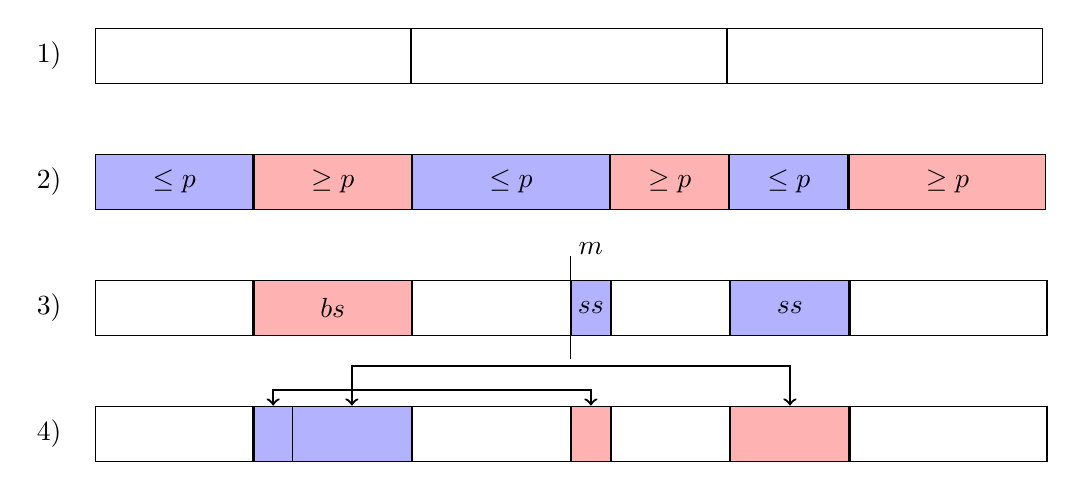
\begin{tikzpicture}[
      node distance = 3mm,
      base/.style={rectangle, draw, minimum height = .7cm},
      small/.style={base,fill=blue!30},
      big/.style={base,fill=red!30},
    ]
      % 1)
      \node (1xl) {1)};
      \node[base, right =     of 1xl, minimum width = 4cm] (1x1) {};
      \node[base, right = 0cm of 1x1, minimum width = 4cm] (1x2) {};
      \node[base, right = 0cm of 1x2, minimum width = 4cm] (1x3) {};


      % 2)
      \node[below = 1cm of 1xl] (2xl) {2)};
      \node[small, right =     of 2xl , minimum width = 2cm] (2x1s) {$\le p$};
      \node[big  , right = 0cm of 2x1s, minimum width = 2cm] (2x1b) {$\ge p$};

      \node[small, right = 0cm of 2x1b, minimum width = 2.5cm] (2x2s) {$\le p$};
      \node[big  , right = 0cm of 2x2s, minimum width = 1.5cm] (2x2b) {$\ge p$};

      \node[small, right = 0cm of 2x2b, minimum width = 1.5cm] (2x3s) {$\le p$};
      \node[big  , right = 0cm of 2x3s, minimum width = 2.5cm] (2x3b) {$\ge p$};

      % 3)
      \node[below = 1cm of 2xl] (3xl) {3)};
      \node[base , right =     of 3xl , minimum width = 2cm] (3x1s) {};
      \node[big  , right = 0cm of 3x1s, minimum width = 2cm] (3x1b) {$bs$};

      \node[base , right = 0cm of 3x1b, minimum width = 2cm]  (3x2s) {};
        % m
      \node[small, right = 0cm of 3x2s, minimum width = .5cm] (3x2sx) {};
      \node[at = (3x2sx.center), anchor=center] {$ss$};


      \node[base , right = 0cm of 3x2sx, minimum width = 1.5cm] (3x2b) {};

      \node[small, right = 0cm of 3x2b, minimum width = 1.5cm] (3x3s) {$ss$};
      \node[base , right = 0cm of 3x3s, minimum width = 2.5cm] (3x3b) {};

      \draw ($ (3x2sx.north west) + (0,.3cm) $) -- ($ (3x2sx.south west) - (0,.3cm) $);
      \node [ above = 2mm of 3x2sx ] {$m$};

      % 4)
      \node[below = 1cm of 3xl] (4xl) {4)};
      \node[base , right =     of 4xl , minimum width = 2cm] (4x1s) {};
      \node[small, right = 0cm of 4x1s, minimum width = 2cm] (4x1b) {};

      \node[base , right = 0cm of 4x1b, minimum width = 2cm]  (4x2s) {};
        % m
      \node[big  , right = 0cm of 4x2s, minimum width = .5cm] (4x2sx) {};
      \node[base , right = 0cm of 4x2sx, minimum width = 1.5cm] (4x2b) {};

      \node[big  , right = 0cm of 4x2b, minimum width = 1.5cm] (4x3s) {};
      \node[base , right = 0cm of 4x3s, minimum width = 2.5cm] (4x3b) {};

      \draw ($ (4x1b.north west) + (.5cm,0) $) -- ($ (4x1b.south west) + (.5cm,0) $);


      \coordinate (swap1left) at ($ (4x1b.north west) + (.25,0) $);
      \draw[<->,thick]
        (swap1left)
        -- ($ (swap1left) + (0,.2) $)
        -- ($ (4x2sx.north) + (0,.2) $)
        -- (4x2sx.north)
        ;

      \coordinate (swap2left) at ($ (4x1b.north west) + (1.25,0) $);
      \draw[<->,thick]
        (swap2left)
        -- ($ (swap2left) + (0,.5) $)
        -- ($ (4x3s.north) + (0,.5) $)
        -- (4x3s.north)
        ;


    \end{tikzpicture}

    \caption{Illustration of the phases of our parallel partitioning algorithm, after a pivot $p$ has been picked.
      Step~1 splits the array into slices. Step~2 partitions the slices in parallel. Step~3 computes the start
      index $m$ of the right partition as the sum of the sizes of all left partitions. It then determines the indexes
      of misplaced elements: the set $bs$ contains right-partition elements that are left of $m$,
      and the set $ss$ contains left partition elements that are right of $m$. Step~4 then swaps the misplaced elements in parallel.
      While Steps~1 and~3 are computationally cheap, Steps~2 and~4 do the main part of the work in parallel.
%
%       1) the array is split into slices,
%       2) the slices are partitioned in parallel. This results into the array consisting of intervals
%       of \emph{small} ($\le p$) and \emph{big} ($\ge p$) elements.
%       3) the size $m$ of the left partition is computed as the sum of all small intervals.
%         This is also the index where the right partition will start in the final result.
%         Then, two sets $ss$ and $bs$ of index intervals are computed, such that $ss$ contains the indexes
%         of small elements that are right of $m$, and $bs$ contains the indexes of big elements left of $m$.
%       4) The elements in $ss$ and $bs$ are swapped in parallel.
    }\label{fig:ppar}
  \end{figure}

  We specify our algorithm on sets of indexes, and then refine it to intervals and interval arrays (cf. Section~\ref{sec:mod_ds}).
  First, we specify Steps~1 and~2, i.e., returning a permutation of the list, along with the sets \is$ls$ of
  indexes that belong to a left partition, and \is$rs$ of indexes that belong to a right partition. In Figure~\ref{fig:ppar},
  \is{ls} corresponds to the set of blue ($\le p$) intervals, and \is$rs$ to the set of red ($\ge p$) intervals:
  \begin{lstlisting}
    ppart_spec p xs == spec (xs',ls,rs).
      mset xs' = mset xs
    & ls \union rs = {0..<|xs'|}  &  ls \inter rs = {}
    & (\<forall>i\<in>ls. xs'!i <= p)  &  (\<forall>i\<in>rs. xs'!i <= p)
  \end{lstlisting}

  The whole partitioning algorithm is specified as follows:
  \begin{lstlisting}
    ppart1 p xs ==
      (xs,ls,rs) <- ppart_spec p xs;   --"\rightcomment{Step 1 and 2}"
      let m = |ls|; ss = {i\<in>ls. m\:<=\:i}; bs = {i\<in>rs. i\:<\:m};   --"\rightcomment{Step 3}"
      xs <- swap_spec ss bs xs;        --"\rightcomment{Step 4}"
      return (m,xs)
  \end{lstlisting}
  A straightforward proof, only using arguments on lists and sets of indexes, shows that this algorithm partitions the list:
  \begin{lstlisting}
  ppart1 p xs <= spec (m, xs').
      mset xs' = mset xs & m <= |xs'| & (\<forall>i<m. xs'!i <= p) & (\<forall>i\<in>{m..<|xs'|}. p <= xs'!i)"
  \end{lstlisting}

  The set operations in Step~3 are implemented by the operations \is{ivo_inter_ivl$_\dagger$} and \is{iv_inter_ivl$_\dagger$} of our interval arrays (cf.~Section~\ref{sec:mod_ds}),
  using the equalities: \is$ {i\<in>ls. m<=i} = {m..} \inter ls$ and \is${i\<in>rs. i<m} = {0..<m} \inter rs$.
  Thus, we are only missing implementations for \is{ppart_spec} and \is{swap_spec}.

  The refinement of the parallel partitioning \is{ppart_spec} is similar to that of the parallel sorting algorithm \is{psort}:
  using \is{with_split} and \is{npar}, we split the list into slices that we then partition with a sequential algorithm.
%   Another technical difficulty we had to solve is the representation of the pivot element: in our original sorting algorithm formalizations, we have always swapped the pivot to the first element of the array, and only passed the index of the pivot element to the partitioning procedure. Now, we actually propagate copies of the pivot element itself to the different parallel partitioning threads. This means that the element type must provide a (deep) copy function. While this is trivial for integers, we had to implement and prove correct such a function for strings.

  The parallel swapping algorithm is refined as follows:
  \begin{lstlisting}
  par_swap ss bs xs ==
    if (ss={}) then return xs
    else xs <- l2o xs; xs <- par_swap_aux ss bs xs; xs <- o2l xs; return xs

  par_swap_aux ss bs xs ==
    ((ss_1,ss_2),(bs_1,bs_2))
      <- spec ((ss_1,ss_2),(bs_1,bs_2)). ss\:=\:ss_1$\dot\cup$ss_2 & bs\:=\:bs_1$\dot\cup$bs_2 & |ss_1|\:=\:|bs_1| & ss_1~={}

    if (ss_2 = {}) then swap_opt_spec ss_1 bs_1 xs
    else
      with_idxs (ss_1 \union bs_1) xs (%xs_1 xs_2.
        (xs_1,xs_2) <- npar swap_opt_spec par_swap_aux (ss_1,bs_1,xs_1) (ss_2,bs_2,xs_2);
        return (xs_1,xs_2)
  \end{lstlisting}
  The main procedure \is{par_swap} first checks if there are any indexes to swap.
  Then, it converts the plain list to a list of option values (\is{l2o}), invokes the actual parallel swapping procedure \is{par_swap_aux},
  and converts the result back to a plain list (\is{o2l}).

  The \is{par_swap_aux} procedure first splits off equally sized, non-empty sets \is{ss_1} and \is{bs_1} from the index sets,
  and then swaps these in parallel with the rest. Here, \is{swap_opt_spec} is the lifting of \is{swap_spec} to lists of option values,
  and \is{with_idxs} ensures that the swap operation will own the necessary elements.

  We prove that our algorithm is correct (\is{par_swap ss bs xs <= swap_spec ss bs xs}),
  and use Sepref, a straightforward implementation of sequential swapping, and our interval array implementation
  to refine it to efficient imperative Isabelle-LLVM code.

  Combining all refinements in this section gives us a parallel partitioning algorithm. When we wanted to show that it
  satisfies the specification \is{partition_spec} as required by our parallel sorting algorithm, we discovered that we
  also need to prove that neither partition can be empty. While this is certainly possible along the same lines as it is proved for sequential partitioning, we chose a pragmatic solution here: we dynamically check for the extreme case of
  one partition being empty, and fix that with an additional swap. The runtime impact of this check is negligible, but it greatly simplifies the correctness proof.




  \subsection{Code Generation}
  Finally, we instantiate the sorting algorithms to sort unsigned integers and strings:
  \begin{lstlisting}
    interpretation unat: cmp (%_. <) (%_. ll_icmp_ult) unat$^{64}_A$ \<proof>
    interpretation str: cmp (%_. <) (%_. strcmp) str$^{64}_A$ \<proof>
  \end{lstlisting}
  Here, the locale \is{cmp} is the version of \is{pcmp} without an extra parameter to the compare function\footnote{
    Parameters to the compare function are currently not supported for parallel sorting algorithms, as we cannot
    efficiently share the parameter between multiple threads. Integrating fractional separation logic into Sepref,
    which would enable such a sharing, is left to future work. }.
  This yields implementations \is{unat.psort$_\dagger$} and \is{str.psort$_\dagger$}, and instantiated versions of the correctness theorem.

  We then use our code generator to generate actual LLVM text, as well as a C header file with the
  signatures of the generated functions\footnote{
    For technical reasons, we represent the array size as non-negative signed integer, thus the C signature uses \lstinline[language=C]{int64_t}.
    Moreover, we use a string implementation based on dynamic arrays, rather than C's zero terminated strings.
  }:
  \begin{lstlisting}
    export_llvm
      unat.psort$_\dagger$ is "uint64_t* psort(uint64_t*, int64_t)"
      str.psort$_\dagger$ is "llstring* str_psort(llstring*, int64_t)"
      defines
        $\textrm{\tt typedef}$ $\textrm{\tt struct}$ {int64_t size; $\textrm{\tt struct}$ {int64_t capacity; char *data;};} llstring;
      file psort.ll
  \end{lstlisting}
  This checks that the specified C signatures are compatible with the actual types, and then
  generates \is{psort.ll} and \is{psort.h}, which can be used in a standard C/C++ toolchain.

%   This can now be compiled, and linked against other C programs using the generated header.
%
%
%   , parametrizing the sorting algorithm over
%   the comparison function
%
%
%
%
%
%   : we take $64$ equidistant samples,
%   and use the median of these samples as pivot.
%
%   Formalization of this sampling algorithm in the Refinement Framework is straightforward.
%   To easily integrate with the existing (highly optimized) implementation of the partitioning algorithm,
%   we have to determine the \emph{index} of the pivot element, swap it with the first element of the array,
%   and then use the existing partitioning algorithm.
%
%   This suggests an algorithm to find the median of a list of sample indexes, comparing each index by looking it up in
%   the list to be sorted, and comparing the corresponding elements.
%   We briefly sketch our approach to formalize such parametrized algorithms using locales, and
%   an extension to Isabelle-LLVM's preprocessor to allow for painless code generation.
%   Note that, for the sake of readability, we have slightly idealized the presentation.
% %   \footnote{
% %     We have omitted some of the fixed parameters, and only describe a parametrized locale.
% %     In practice, we have two versions of the locale, one with a parameter, and one without. While they are still based on the same abstract algorithms, they duplicate some boilerplate code.
% %   }.
%
%
%   A \emph{locale}~\cite{KWP99} is a named context that fixes some parameters and makes assumptions about these parameters.
%   Inside a locale, definitions and theorems can depend on the parameters and assumptions.
%   Later, a locale can be instantiated with actual terms for the parameters, proving that they satisfy the assumptions.
%   This makes available instantiated versions of the definitions and theorems proved inside the locale.
%   Instantiations can also be nested, that is, a locale can be instantiated in the context of another locale.
%
%   We define a locale to set up a parametrized compare function as follows:
%   \begin{lstlisting}
%     locale pcmp =
%       fixes lt lti par$_A$ elem$_A$
%       assumes weak_ordering (lt p)
%       assumes hnr
%         (par$_A$ p pi * elem$_A$ a ai * elem$_A$ b bi)
%         (lti pi ai bi)
%         (par$_A$ p pi * elem$_A$ a ai * elem$_A$ b bi)  (bool$_A$)  (%_. True)
%         (lt p a b)
%
%   \end{lstlisting}
%   that is, we fix an abstract compare function \is{lt}. It takes one extra parameter \is{p},
%   and is a weak ordering\footnote{
%     A weak ordering can be defined by mapping the elements into a total ordering, and is the standard prerequisite for sorting algorithms in C++~\cite{Josu12}.
%   } for each such \is{p}. We also fix a concrete compare function \is{lti}, that refines the abstract compare
%   function, with refinement assertion \is{par$_A$} for the parameter, and \is{elem$_A$} for the elements to be sorted.
%
%   Inside the \is{pcmp} locale, we define our sorting and median functions, threading through the explicit parameter \is{p}.
%   Among others, this will yield a function \is{median p xs}, which returns the median index of the elements in list \is{xs},
%   comparing wrt.\ \is{lt p}. We also get a corresponding implementation \is{median_impl}\footnote{We simply reused a sequential sorting algorithm to completely sort the list and then obtain the middle element. While this is not the most efficient way of finding a median, the overhead when sorting $64$ element arrays is negligible compared to the time spent for sorting the partitions that are at least $10^5$ elements large. Thus, a more efficient algorithm like quickselect would not have any measurable effect on the overall performance, and we leave its verification to future work.}.
%
%   To implement the sampling algorithm, \is{inside} the \is{pcmp} locale, we define
%   a comparison function for indexes, parametrized with the original parameter and the array to be sorted.
%   For this, we instantiate the \is{pcmp} locale again\footnote{In the actual formalization, we use a slightly more complex locale hierarchy to carefully avoid infinite recursive instantiations.}:
%   \begin{lstlisting}
%     context pcmp begin
%
%       definition "lt_idx (p,xs) i j == lt p (xs!i) (xs!j)"
%       definition "lt_idx_impl == ..."
%
%       sublocale IDX: pcmp lt_idx lt_idx_impl (par$_A$ \<times> arr$_A$) idx$_A$   \<proof>
%   \end{lstlisting}
%   This makes available a function \is{IDX.median} and its implementation, which compares indexes into arrays as desired.
%   This is then used in the partitioning function.
%
%   Next, the \is{pcmp} locale is instantiated globally, for example to sort unsigned integers:
%   \begin{lstlisting}
%     global_interpretation unat: pcmp (<) ll_icmp_ult unat$^{64}_A$ \<proof>
%   \end{lstlisting}
%   The \is{global_interpretation} command instantiates the locale for comparing natural
%   numbers implemented by 64 bit words (\is{unat$^{64}_A$}). It yields a proof obligation that
%   the LLVM instruction \is{ll_icmp_ult} actually implements the \is{(<)} operation on natural numbers,
%   which is easily discharged.
%

%
%
%
%
%   For the sake of clarity, we have omitted the fact that our whole development so far has been parametrized
%   over a weak ordering, and a refinement assertion for the array elements.
%   A weak ordering is any ordering induced by a mapping into a total ordering.
%   It is the standard requirement for compare operations used for sorting in C++~\cite{Josu12}.
%   Before we can generate LLVM code, we have to instantiate the compare operator accordingly.
%   For example, to sort natural numbers implemented by unsigned integers (\is{unat$_A$}), we instantiate:
%   \begin{lstlisting}
%     global_interpretation unat: sort_impl_context "(<)" ll_icmp_ult unat$_A$
%   \end{lstlisting}
%   This yields a proof obligation that the LLVM instruction \is{ll_icmp_ult} on LLVM integers
%   actually implements the \is{(<)} operation on natural numbers, wrt.\ the refinement assertion \is{unat$_A$},
%   which is easily discharged. We then get instantiated versions of \is{psort$_\dagger$}, and also of the correctness theorem.
%
%   In a last step, we use our code generator to generate actual LLVM text, as well as a C header file with the
%   signatures of the generated functions\footnote{
%     For technical reasons, we represent the array size as non-negative signed integer, thus the second argument of the C signature has
%     the signed type \lstinline[language=C]{int64_t}.
%   }:
%   \begin{lstlisting}
%     export_llvm unat.psort$_\dagger$ is "uint64_t* psort(uint64_t*, int64_t)" file psort.ll
%   \end{lstlisting}
%   This can now be compiled, and linked against other C programs using the generated header.
%   A similar instantiation is done for the lexicographic ordering on strings, represented by dynamic arrays of bytes.
%


%
%
%
%
%
%
%
%
%   the partition gets too small, or the recursion too deep
%
%
%
%
%   That is, for a valid range of indexes \is{l..<h}, the new list is a permutation of the old list,
%   equal to the old list outside the range, and sorted inside the range.
%
%
%   Our version of the Sepref tool is mostly backwards compatible with the original Sepref tool for Isabelle-LLVM~\cite{La19-llvm}.
%   The only difference is the handling of concrete pointer equalities (cf.\ Section~\ref{sec::array_split}).
%   Thus, it was a mainly straightforward task to port the efficient verified Introsort and pdqsort algorithms~\cite{La20} to the new tool,
%   additionally proving that the concrete algorithm is in-place, i.e., the returned array pointer equals the argument pointer.
%   Equipped with these refinements, the Sepref tool can synthesize a parallel sorting algorithm from \is{sort_aux} (Section~\ref{sec:sortspec}), using the already existing partitioning algorithm and the
%   pdqsort algorithm for the abstract \is{partition_spec} and \is{sort_spec} specifications.
%
%   Actually, we used refinement steps on the abstract level to add two optimizations:
%   first, we add an explicit parameter for the length of the list. This allows us to refine the list
%   to just an array pointer\footnote{Alternatively, we could refine a list to a pair of array pointer and explicit length.}.
%   Second, to prevent creation of parallel threads for small partitions, we proceed sequentially if the created partitions
%   are too unbalanced. The following is the algorithm that we input into Sepref\footnote{We have omitted some
%   of the assertions required to prove that the arithmetic operations do not overflow.}:
%   \begin{lstlisting}
%     psort_aux xs n d ==
%       assert n=|xs|
%       if d=0 \or n<100000 then {
%         slice_sort_spec xs 0 n
%       } else {
%         (xs,m) <- slice_partition_spec xs 0 n;
%         let bad = m<n div 8 \or (n-m < n div 8)
%         (_,xs) <- with_split m xs (%xs_1 xs_2. {
%           if bad then nseq psort_aux psort_aux (xs_1,m,d-1) (xs_2,n-m,d-1)
%           else npar psort_aux psort_aux (xs_1,m,d-1) (xs_2,n-m,d-1)
%         });
%         return xs
%       }"
%
%     nseq f_1 f_2 x_1 x_2 == r_1 <- f_1 x_1; r_2 <- f_2 x_2; return (x_1,x_2)
%
%     psort xs n ==
%       assert n=|xs|
%       if n<=1 then return xs
%       else psort_aux xs n (log2 n * 2)
%
%   \end{lstlisting}
%   where \is{nseq} is abstractly the same as \is{npar}, but is translated to sequential execution by the Sepref tool.
%   Moreover, \is{slice_sort_spec} and \is{slice_partition_spec} are the specifications for sorting and partitioning
%   only a slice of the array, leaving the rest unchanged. These match the interface of the original sequential algorithms
%   proved correct in~\cite{La20}. Finally, \is{psort} wraps the algorithm to run with an initial depth limit of $2\lfloor\log_2 n\rfloor$.

%   \subsection{A Sampling Partitioner}
%   While we could simply re-use the existing partitioning algorithm from the Introsort formalization,
%   which uses a median-of-three pivot selection, we observe that the quality of the pivot is
%   particularly important for a balanced parallelization. Moreover, the partitioning in the \is{psort_aux} procedure
%   is only done for arrays above a quite big size threshold. Thus, we can invest a little more work to find
%   a good pivot, which is still negligible compared to the cost of sorting the resulting partitions.
%
%   We choose a rather simple sampling approach: for an array of size $n$, we take $\min(n,64)$ equidistant samples,
%   and use the median of these samples as pivot.
%
%   Formalization of this sampling algorithm in the Refinement Framework is straightforward.
%   To easily integrate with the existing (highly optimized) implementation of the partitioning algorithm,
%   we have to determine the \emph{index} of the pivot element, swap it with the first element of the array,
%   and then use the existing partitioning algorithm.
%
%   This suggests an algorithm to find the median of a list of sample indexes, comparing each index by looking it up in
%   the list to be sorted, and comparing the corresponding elements.
%   We briefly sketch our approach to formalize such parametrized algorithms using locales, and
%   an extension to Isabelle-LLVM's preprocessor to allow for painless code generation.
%   Note that, for the sake of readability, we have slightly idealized the presentation\footnote{
%     We have omitted some of the fixed parameters, and only describe a parametrized locale.
%     In practice, we have two versions of the locale, one with a parameter, and one without. While they are still based on the same abstract algorithms, they duplicate some boilerplate code.
%   }.
%
%   A \emph{locale}~\cite{KWP99} is a named context that fixes some parameters and makes assumptions about these parameters.
%   Inside a locale, definitions and theorems can depend on the parameters and assumptions.
%   Later, a locale can be instantiated with actual terms for the parameters, proving that they satisfy the assumptions.
%   This makes available instantiated versions of the definitions and theorems proved inside the locale.
%   Instantiations can also be nested, that is, a locale can be instantiated in the context of another locale.
%
%   We define a locale to set up a parametrized compare function as follows:
%   \begin{lstlisting}
%     locale pcmp =
%       fixes lt lti par$_A$ elem$_A$
%       assumes weak_ordering (lt p)
%       assumes hnr
%         (par$_A$ p pi * elem$_A$ a ai * elem$_A$ b bi)
%         (lti pi ai bi)
%         (par$_A$ p pi * elem$_A$ a ai * elem$_A$ b bi)  (bool$_A$)  (%_. True)
%         (lt p a b)
%
%   \end{lstlisting}
%   that is, we fix an abstract compare function \is{lt}. It takes one extra parameter \is{p},
%   and is a weak ordering\footnote{
%     A weak ordering can be defined by mapping the elements into a total ordering, and is the standard prerequisite for sorting algorithms.
%   } for each such \is{p}. We also fix a concrete compare function \is{lti}, that refines the abstract compare
%   function, with refinement assertion \is{par$_A$} for the parameter, and \is{elem$_A$} for the elements to be sorted.
%
%   Inside the \is{pcmp} locale, we define our sorting and median functions, threading through the explicit parameter \is{p}.
%   Among others, this will yield a function \is{median p xs}, which returns the median index of the elements in list \is{xs},
%   comparing wrt.\ \is{lt p}. We also get a corresponding implementation \is{median_impl}\footnote{We simply reused a sequential sorting algorithm to completely sort the list and then obtain the middle element. While this is not the most efficient way of finding a median, the overhead when sorting $64$ element arrays is negligible compared to the time spent for sorting the partitions that are at least $10^5$ elements large. Thus, a more efficient algorithm like quickselect would not have any measurable effect on the overall performance, and we leave its verification to future work.}.
%
%   To implement the sampling algorithm, \is{inside} the \is{pcmp} locale, we define
%   a comparison function for indexes, parametrized with the original parameter and the array to be sorted.
%   For this, we instantiate the \is{pcmp} locale again\footnote{In the actual formalization, we use a slightly more complex locale hierarchy to carefully avoid infinite recursive instantiations.}:
%
%   \begin{lstlisting}
%     context pcmp begin
%
%       definition "lt_idx (p,xs) i j == lt p (xs!i) (xs!j)"
%       definition "lt_idx_impl == ..."
%
%       sublocale IDX: pcmp lt_idx lt_idx_impl (par$_A$ \<times> arr$_A$) idx$_A$   \<proof>
%
%   \end{lstlisting}
%   This makes available a function \is{IDX.median} and its implementation, which compares indexes into arrays as desired.
%   This is then used in the partitioning function.
%
%   Finally, the \is{pcmp} locale is instantiated globally, for example to sort unsigned integers, and the resulting implementation is
%   exported to LLVM text:
%   \begin{lstlisting}
%     global_interpretation unat: pcmp (<) ll_icmp_ult unat$^{64}_A$   \<proof>
%
%     export_llvm unat.psort$_\dagger$
%   \end{lstlisting}
%   The \is{global_interpretation} command instantiates the locale for comparing natural
%   numbers implemented by 64 bit words (\is{unat$^{64}_A$}). Note that the compare function is not
%   parametrized. Finally, the \is{export_llvm} command generates LLVM text.
%   It first uses a preprocessor to generate and prove correct a set of code equations, which are then pretty printed to actual LLVM text.
%   The preprocessor does not contribute to the trusted code base, as it proves correct its transformations.
%   At this point, we have added a transformation to automatically instantiate the higher-order parameters generated by Isabelle's locale mechanism.
%   This saves a lot of boilerplate code that was necessary in the original sorting algorithm formalization~\cite{La20}, and became unmanageable
%   once we added the sublocale for comparing indexes into an array.


%
%   xxx: array splitting
%
%   then short explanation that proofs are semi-automatic.
%
%
%   also mention optimizations of algorithm (bad-partition)
%
%
%
%   Sepref comes with standard setup to refine lists to arrays. List updates are refined to destructive array updates,
%   as long as the old version of the list is not used after the update.
%   It also provides setup to refine unbounded natural numbers to bounded integers.
%   It tries to discharge the resulting in-bounds proof obligations automatically.
%   If this is not possible, it relies on hints from the user.
%
%
%     - intro to sepref
%     - parallel hnr rule
%     - identity tracking
%     - array splitting

%   \section{Parallel Quicksort}
%   \subsection{The Algorithm}
%
%   \subsection{Array Data Structure}




%   \subsection{Final Implementation and Correctness Theorem}
%   From this algorithm, the Sepref tool generates an imperative implementation \is{psort$_\dagger$} and proves the corresponding \is{hnr} refinement lemma.
%   Finally, our code generator translates \is{psort$_\dagger$} to an LLVM function.
%   Combining the refinement lemma with the correctness lemma of the abstract \is{psort} algorithm, and unfolding the definition of \is{hnr},
%   we get the following Hoare-triple, that states correctness of our final algorithm:
%   \begin{lstlisting}
%   "ht (arr$_A$ xs xsi * idx$_A$ n ni * n = |xs|)
%     (psort$_\dagger$ xsi ni)
%     (%r. r=xsi * \<exists> xs'. arr$_A$ xs' xsi * sorted xs' * mset xs' = mset xs)"
%   \end{lstlisting}
%   That is, for a pointer \is{xsi} to an array, whose contents are described by list \is{xs} (\is{arr$_A$}), and a fixed-size word \is{ni} representing the natural number \is{n} (\is{idx$_A$}),
%   which must be the number of elements in the list \is{xs}, our sorting algorithm returns the original pointer \is{xsi}, and the array contents are now \is{xs'},
%   which is sorted and a permutation of \is{xs}.
%   Note that, while the trusted code base of this statement includes our LLVM semantics and code generator, as well as Isabelle's inference kernel,
%   it does not include the refinement steps, verification condition generation, Hoare-rules, or automated theorem provers invoked by sledgehammer~\cite{BBP13},
%   which we used to prove this statement.
%






























%
%
%   \subsection{Specification of Sorting Algorithms}\label{sec:sortspec}
%   The first step to verify a sorting algorithm is to specify the desired result.
%   We specify an algorithm that sorts a list \is{xs} as follows:
%   \begin{lstlisting}
%     sort_spec xs == spec xs'. sorted xs' \and mset xs' = mset xs
%   \end{lstlisting}
%   where \is{mset xs} is the multiset of the elements in the list \is{xs}.
%   That is, the resulting list \is{xs'} is sorted, and a permutation of the original list \is{xs}.
%
%   For quicksort-like sorting algorithms, the main function is partitioning, which reshuffles a
%   given list into two partitions, such that any element in the first partition is less than or equal
%   to any element in the second partition. We specify a partitioning function that assumes at least four elements,
%   and is guaranteed to return non-empty partitions. The result is returned as a reshuffled list \is{xs'},
%   and the index \is{m} of the first element of the second partition:
%   \begin{lstlisting}
%     partition_spec xs = assert (4 <= length xs);
%       spec (xs',m). mset xs' = mset xs \and 0<m \and m<|xs|
%       \and (\<forall>i\<in>{0..<m}. \<forall>j\<in>{m..<|xs|}. xs'!i <= xs'!j)
%   \end{lstlisting}
%
%   Using the above specifications as building blocks, we can define a simple abstract sorting algorithm:
%   \begin{lstlisting}
%     sort_aux xs d ==
%       if d=0 \or |xs|<100000 then { --"\rightcomment{check depth bound or size threshold}"
%         sort_spec xs --"\rightcomment{sort with some (sequential) algorithm}"
%       } else {
%         (xs,m) <- partition_spec xs;  --"\rightcomment{partition}"
%         with_split m xs (%xs_1 xs_2. { --"\rightcomment{work on partitions $xs_1$ and $xs_2$}"
%           npar sort_aux sort_aux (xs_1,d-1) (xs_2,d-1) --"\rightcomment{recursively sort in parallel}"
%         })
%       }"
%   \end{lstlisting}
%   where
%   \begin{lstlisting}
%     with_split m xs f ==
%       assert (m < |xs|);
%       (xs_1,xs_2) <- f (take m xs) (drop m xs);
%       assert (|xs_1| = m \and |xs_2| = |xs| - m);
%       return (xs_1@xs_2)
%
%     npar f g x y == r1 <- f x; r2 <- g y; return (r1,r2)
%   \end{lstlisting}
%   where \is{@} appends two lists.
%   This algorithm is derived from Introsort~\cite{Muss97}, a quicksort with a depth bound to ensure $O(n\log n)$ worst-case complexity.
%   If the recursion depth bound $d$ is reached, or the list size is below a certain threshold,
%   we sort the list using some yet unspecified sorting algorithm. Otherwise, we partition the list
%   and recursively sort the two partitions.
%
%   Here, we have introduced two new combinators,
%   which are hints for the following refinement steps: (1) the \is{with_split} combinator splits a given list into two parts,
%   and invokes a function that can change the content of these two parts, but not their length. It then returns
%   the concatenation of the two changed parts. It is a hint for the further refinement steps to implement the list as
%   an array that is modified in-place. (2) the \is{npar} combinator simply executes two blocks sequentially.
%   Note that, for our stateless abstract programs, there is no difference between parallel and (independent) sequential execution.
%   However, \is{npar} is a hint to the subsequent refinement steps to refine to parallel execution.
%
%   Using the tools of the Isabelle Refinement Framework~\cite{LaTu12}, and some existing theories copied from~\cite{La19-llvm},
%   it is straightforward to prove that this sorting algorithm is correct, i.e.:
%   \begin{lstlisting}
%     sort_aux xs d <= sort_spec xs
%   \end{lstlisting}
%
%   In the next sections, we will explain how to refine this two an actual parallel sorting algorithm in LLVM,
%   re-using the existing sequential pdqsort algorithm~\cite{La19-llvm} for small or too deep partitions, and a sampling algorithm for finding good pivots for partitioning.
%
%
%
%   \section{A Parallel Sorting Algorithm}\label{sec:parsort}
%   Our version of the Sepref tool is mostly backwards compatible with the original Sepref tool for Isabelle-LLVM~\cite{La19-llvm}.
%   The only difference is the handling of concrete pointer equalities (cf.\ Section~\ref{sec::array_split}).
%   Thus, it was a mainly straightforward task to port the efficient verified Introsort and pdqsort algorithms~\cite{La20} to the new tool,
%   additionally proving that the concrete algorithm is in-place, i.e., the returned array pointer equals the argument pointer.
%   Equipped with these refinements, the Sepref tool can synthesize a parallel sorting algorithm from \is{sort_aux} (Section~\ref{sec:sortspec}), using the already existing partitioning algorithm and the
%   pdqsort algorithm for the abstract \is{partition_spec} and \is{sort_spec} specifications.
%
%   Actually, we used refinement steps on the abstract level to add two optimizations:
%   first, we add an explicit parameter for the length of the list. This allows us to refine the list
%   to just an array pointer\footnote{Alternatively, we could refine a list to a pair of array pointer and explicit length.}.
%   Second, to prevent creation of parallel threads for small partitions, we proceed sequentially if the created partitions
%   are too unbalanced. The following is the algorithm that we input into Sepref\footnote{We have omitted some
%   of the assertions required to prove that the arithmetic operations do not overflow.}:
%   \begin{lstlisting}
%     psort_aux xs n d ==
%       assert n=|xs|
%       if d=0 \or n<100000 then {
%         slice_sort_spec xs 0 n
%       } else {
%         (xs,m) <- slice_partition_spec xs 0 n;
%         let bad = m<n div 8 \or (n-m < n div 8)
%         (_,xs) <- with_split m xs (%xs_1 xs_2. {
%           if bad then nseq psort_aux psort_aux (xs_1,m,d-1) (xs_2,n-m,d-1)
%           else npar psort_aux psort_aux (xs_1,m,d-1) (xs_2,n-m,d-1)
%         });
%         return xs
%       }"
%
%     nseq f_1 f_2 x_1 x_2 == r_1 <- f_1 x_1; r_2 <- f_2 x_2; return (x_1,x_2)
%
%     psort xs n ==
%       assert n=|xs|
%       if n<=1 then return xs
%       else psort_aux xs n (log2 n * 2)
%
%   \end{lstlisting}
%   where \is{nseq} is abstractly the same as \is{npar}, but is translated to sequential execution by the Sepref tool.
%   Moreover, \is{slice_sort_spec} and \is{slice_partition_spec} are the specifications for sorting and partitioning
%   only a slice of the array, leaving the rest unchanged. These match the interface of the original sequential algorithms
%   proved correct in~\cite{La20}. Finally, \is{psort} wraps the algorithm to run with an initial depth limit of $2\lfloor\log_2 n\rfloor$.
%
% %   \subsection{A Sampling Partitioner}
% %   While we could simply re-use the existing partitioning algorithm from the Introsort formalization,
% %   which uses a median-of-three pivot selection, we observe that the quality of the pivot is
% %   particularly important for a balanced parallelization. Moreover, the partitioning in the \is{psort_aux} procedure
% %   is only done for arrays above a quite big size threshold. Thus, we can invest a little more work to find
% %   a good pivot, which is still negligible compared to the cost of sorting the resulting partitions.
% %
% %   We choose a rather simple sampling approach: for an array of size $n$, we take $\min(n,64)$ equidistant samples,
% %   and use the median of these samples as pivot.
% %
% %   Formalization of this sampling algorithm in the Refinement Framework is straightforward.
% %   To easily integrate with the existing (highly optimized) implementation of the partitioning algorithm,
% %   we have to determine the \emph{index} of the pivot element, swap it with the first element of the array,
% %   and then use the existing partitioning algorithm.
% %
% %   This suggests an algorithm to find the median of a list of sample indexes, comparing each index by looking it up in
% %   the list to be sorted, and comparing the corresponding elements.
% %   We briefly sketch our approach to formalize such parametrized algorithms using locales, and
% %   an extension to Isabelle-LLVM's preprocessor to allow for painless code generation.
% %   Note that, for the sake of readability, we have slightly idealized the presentation\footnote{
% %     We have omitted some of the fixed parameters, and only describe a parametrized locale.
% %     In practice, we have two versions of the locale, one with a parameter, and one without. While they are still based on the same abstract algorithms, they duplicate some boilerplate code.
% %   }.
% %
% %   A \emph{locale}~\cite{KWP99} is a named context that fixes some parameters and makes assumptions about these parameters.
% %   Inside a locale, definitions and theorems can depend on the parameters and assumptions.
% %   Later, a locale can be instantiated with actual terms for the parameters, proving that they satisfy the assumptions.
% %   This makes available instantiated versions of the definitions and theorems proved inside the locale.
% %   Instantiations can also be nested, that is, a locale can be instantiated in the context of another locale.
% %
% %   We define a locale to set up a parametrized compare function as follows:
% %   \begin{lstlisting}
% %     locale pcmp =
% %       fixes lt lti par$_A$ elem$_A$
% %       assumes weak_ordering (lt p)
% %       assumes hnr
% %         (par$_A$ p pi * elem$_A$ a ai * elem$_A$ b bi)
% %         (lti pi ai bi)
% %         (par$_A$ p pi * elem$_A$ a ai * elem$_A$ b bi)  (bool$_A$)  (%_. True)
% %         (lt p a b)
% %
% %   \end{lstlisting}
% %   that is, we fix an abstract compare function \is{lt}. It takes one extra parameter \is{p},
% %   and is a weak ordering\footnote{
% %     A weak ordering can be defined by mapping the elements into a total ordering, and is the standard prerequisite for sorting algorithms.
% %   } for each such \is{p}. We also fix a concrete compare function \is{lti}, that refines the abstract compare
% %   function, with refinement assertion \is{par$_A$} for the parameter, and \is{elem$_A$} for the elements to be sorted.
% %
% %   Inside the \is{pcmp} locale, we define our sorting and median functions, threading through the explicit parameter \is{p}.
% %   Among others, this will yield a function \is{median p xs}, which returns the median index of the elements in list \is{xs},
% %   comparing wrt.\ \is{lt p}. We also get a corresponding implementation \is{median_impl}\footnote{We simply reused a sequential sorting algorithm to completely sort the list and then obtain the middle element. While this is not the most efficient way of finding a median, the overhead when sorting $64$ element arrays is negligible compared to the time spent for sorting the partitions that are at least $10^5$ elements large. Thus, a more efficient algorithm like quickselect would not have any measurable effect on the overall performance, and we leave its verification to future work.}.
% %
% %   To implement the sampling algorithm, \is{inside} the \is{pcmp} locale, we define
% %   a comparison function for indexes, parametrized with the original parameter and the array to be sorted.
% %   For this, we instantiate the \is{pcmp} locale again\footnote{In the actual formalization, we use a slightly more complex locale hierarchy to carefully avoid infinite recursive instantiations.}:
% %
% %   \begin{lstlisting}
% %     context pcmp begin
% %
% %       definition "lt_idx (p,xs) i j == lt p (xs!i) (xs!j)"
% %       definition "lt_idx_impl == ..."
% %
% %       sublocale IDX: pcmp lt_idx lt_idx_impl (par$_A$ \<times> arr$_A$) idx$_A$   \<proof>
% %
% %   \end{lstlisting}
% %   This makes available a function \is{IDX.median} and its implementation, which compares indexes into arrays as desired.
% %   This is then used in the partitioning function.
% %
% %   Finally, the \is{pcmp} locale is instantiated globally, for example to sort unsigned integers, and the resulting implementation is
% %   exported to LLVM text:
% %   \begin{lstlisting}
% %     global_interpretation unat: pcmp (<) ll_icmp_ult unat$^{64}_A$   \<proof>
% %
% %     export_llvm unat.psort$_\dagger$
% %   \end{lstlisting}
% %   The \is{global_interpretation} command instantiates the locale for comparing natural
% %   numbers implemented by 64 bit words (\is{unat$^{64}_A$}). Note that the compare function is not
% %   parametrized. Finally, the \is{export_llvm} command generates LLVM text.
% %   It first uses a preprocessor to generate and prove correct a set of code equations, which are then pretty printed to actual LLVM text.
% %   The preprocessor does not contribute to the trusted code base, as it proves correct its transformations.
% %   At this point, we have added a transformation to automatically instantiate the higher-order parameters generated by Isabelle's locale mechanism.
% %   This saves a lot of boilerplate code that was necessary in the original sorting algorithm formalization~\cite{La20}, and became unmanageable
% %   once we added the sublocale for comparing indexes into an array.
%
%
% %
% %   xxx: array splitting
% %
% %   then short explanation that proofs are semi-automatic.
% %
% %
% %   also mention optimizations of algorithm (bad-partition)
% %
% %
% %
% %   Sepref comes with standard setup to refine lists to arrays. List updates are refined to destructive array updates,
% %   as long as the old version of the list is not used after the update.
% %   It also provides setup to refine unbounded natural numbers to bounded integers.
% %   It tries to discharge the resulting in-bounds proof obligations automatically.
% %   If this is not possible, it relies on hints from the user.
% %
% %
% %     - intro to sepref
% %     - parallel hnr rule
% %     - identity tracking
% %     - array splitting
%
% %   \section{Parallel Quicksort}
% %   \subsection{The Algorithm}
% %
% %   \subsection{Array Data Structure}
%
%
%
%
%   \subsection{Final Implementation and Correctness Theorem}
%   From this algorithm, the Sepref tool generates an imperative implementation \is{psort$_\dagger$} and proves the corresponding \is{hnr} refinement lemma.
%   Finally, our code generator translates \is{psort$_\dagger$} to an LLVM function.
%   Combining the refinement lemma with the correctness lemma of the abstract \is{psort} algorithm, and unfolding the definition of \is{hnr},
%   we get the following Hoare-triple, that states correctness of our final algorithm:
%   \begin{lstlisting}
%   "ht (arr$_A$ xs xsi * idx$_A$ n ni * n = |xs|)
%     (psort$_\dagger$ xsi ni)
%     (%r. r=xsi * \<exists> xs'. arr$_A$ xs' xsi * sorted xs' * mset xs' = mset xs)"
%   \end{lstlisting}
%   That is, for a pointer \is{xsi} to an array, whose contents are described by list \is{xs} (\is{arr$_A$}), and a fixed-size word \is{ni} representing the natural number \is{n} (\is{idx$_A$}),
%   which must be the number of elements in the list \is{xs}, our sorting algorithm returns the original pointer \is{xsi}, and the array contents are now \is{xs'},
%   which is sorted and a permutation of \is{xs}.
%   Note that, while the trusted code base of this statement includes our LLVM semantics and code generator, as well as Isabelle's inference kernel,
%   it does not include the refinement steps, verification condition generation, Hoare-rules, or automated theorem provers invoked by sledgehammer~\cite{BBP13},
%   which we used to prove this statement.
%

  \subsection{Benchmarks}\label{sec:benchmark}
  \newcommand{\plottim}[4]{
  \begin{tikzpicture}
    \begin{axis}[
      ymajorgrids,
      title={\large #1},
      title style={at={(0.12,.75)}},
      ybar=0pt,
      width=\textwidth,
      height=.249\textheight,
      bar width=2.5pt,
      xtick=data,
      symbolic x coords={rev-sorted-end-10,rev-sorted-end-1,sorted-end-.1,almost-sorted-50,random-boolean,organ-pipe,sorted-end-10,equal,rev-sorted-middle-.1,rev-sorted,sorted-middle-1,rev-sorted-middle-10,random,almost-sorted-.1,sorted,rev-sorted-middle-1,sorted-middle-.1,almost-sorted-10,almost-sorted-1,sorted-middle-10,rev-sorted-end-.1,sorted-end-1,random-dup-10,}
      ,
      #3
    ]

      \input{#2}

      \addplot[black, thin, sharp plot,update limits=false]
	coordinates {([normalized]-10,1) ([normalized]100,1)};
% 	node[above] at (axis cs:1950,4.3e7) {Houses};
      #4
    \end{axis}
  \end{tikzpicture}
  }

  \begin{figure}
    \plottim{Laptop, uint64}{data_laptop_uint64}{xticklabels={},ytick distance={200}}{\legend{}}
    \plottim{Server, uint64}{data_server_uint64}{xticklabels={},ytick distance={200},ymax=1100}{\legend{}}
    \plottim{Laptop, string}{data_laptop_llstring}{xticklabels={},ytick distance={200},ymax=1100}{\legend{}}
    \plottim{Server, string}{data_server_llstring}{
      xlabel near ticks, x tick label style={rotate=45,anchor=east,font=\tiny},
      ytick distance={200},ymax=1000,
      legend style = {
%         legend pos= north east,
        at = {(.77,.97)},
        cells={anchor=west},
        font=\tiny
      },
    }{}

  \caption{Runtimes in milliseconds for sorting various distributions of $10^8$ unsigned 64 bit integers and $10^7$ strings with
    our verified parallel sorting algorithm, C++'s standard parallel sorting algorithm, and Boost's parallel sample sort algorithm.
    The experiments were performed on a server machine with 22 AMD Opteron 6176 cores and 128GiB of RAM, and a laptop with a
    6 core (12 threads) i7-10750H CPU and 32GiB of RAM.
  }\label{fig:benchres}
  \end{figure}


  \begin{figure}

  \begin{tikzpicture}
    \begin{axis}[
      xlabel near ticks,
      legend style = {
        at = {(.97,.35)},
        cells={anchor=west},
        font=\tiny
      },
      ymajorgrids,
      xmin=1, ymin=1, xmax=12, ymax=8,
      title={\large Laptop (u64)},
      title style={at={(0.25,.75)}},
      width=.54\textwidth,
      height=.3\textheight
    ]
      
\addplot+[color=red, mark color=black, mark options={fill=red}] coordinates {
  (1, 1.00)
  (2, 1.81)
  (3, 2.68)
  (4, 3.52)
  (5, 4.35)
  (6, 5.15)
  (7, 5.51)
  (8, 5.95)
  (9, 6.14)
  (10, 6.34)
  (11, 6.87)
  (12, 6.72)
};
\addlegendentry{verified};

\addplot+[color=black, mark color=black, mark options={fill=black}] coordinates {
  (1, 1.00)
  (2, 1.92)
  (3, 2.84)
  (4, 3.73)
  (5, 4.55)
  (6, 5.31)
  (7, 5.79)
  (8, 6.20)
  (9, 6.29)
  (10, 6.42)
  (11, 6.60)
  (12, 6.85)
};
\addlegendentry{sample sort};

\addplot+[color=blue, mark color=black, mark options={fill=blue}] coordinates {
  (1, 1.00)
  (2, 1.93)
  (3, 2.86)
  (4, 3.79)
  (5, 4.70)
  (6, 5.55)
  (7, 5.99)
  (8, 6.38)
  (9, 6.74)
  (10, 7.11)
  (11, 7.35)
  (12, 7.61)
};
\addlegendentry{std::sort};


      \draw[black, thin, sharp plot]
      (axis cs:\pgfkeysvalueof{/pgfplots/xmin},\pgfkeysvalueof{/pgfplots/xmin}) --
      (axis cs:\pgfkeysvalueof{/pgfplots/xmax},\pgfkeysvalueof{/pgfplots/xmax});


%       \addplot[black, thin, sharp plot, update limits=false] {\x};
    \end{axis}
  \end{tikzpicture}\hfill
  \begin{tikzpicture}
    \begin{axis}[
      xlabel near ticks,
      legend style = {
        at = {(.87,.3)},
        cells={anchor=west},
        font=\scriptsize
      },
      ymajorgrids,
      xmin=1, ymin=1, xmax=12, ymax=8,
      title={\large Laptop (str)},
      title style={at={(0.25,.75)}},
      width=.54\textwidth,
      height=.3\textheight
    ]
      
\addplot+[color=red, mark color=black, mark options={fill=red}] coordinates {
  (1, 1.00)
  (2, 1.83)
  (3, 2.52)
  (4, 3.03)
  (5, 3.42)
  (6, 3.67)
  (7, 3.92)
  (8, 3.95)
  (9, 4.20)
  (10, 4.19)
  (11, 4.54)
  (12, 4.65)
};
\addlegendentry{verified};

\addplot+[color=black, mark color=black, mark options={fill=black}] coordinates {
  (1, 1.00)
  (2, 1.92)
  (3, 2.72)
  (4, 3.37)
  (5, 3.90)
  (6, 4.17)
  (7, 4.30)
  (8, 4.43)
  (9, 4.58)
  (10, 4.69)
  (11, 4.71)
  (12, 4.79)
};
\addlegendentry{sample sort};

\addplot+[color=blue, mark color=black, mark options={fill=blue}] coordinates {
  (1, 1.00)
  (2, 1.75)
  (3, 2.37)
  (4, 2.84)
  (5, 3.17)
  (6, 3.18)
  (7, 3.48)
  (8, 3.52)
  (9, 3.74)
  (10, 3.87)
  (11, 4.08)
  (12, 4.14)
};
\addlegendentry{std::sort};


      \draw[black, thin, sharp plot]
      (axis cs:\pgfkeysvalueof{/pgfplots/xmin},\pgfkeysvalueof{/pgfplots/xmin}) --
      (axis cs:\pgfkeysvalueof{/pgfplots/xmax},\pgfkeysvalueof{/pgfplots/xmax});

      \legend{}

%       \addplot[black, thin, sharp plot, update limits=false] {\x};
    \end{axis}
  \end{tikzpicture}\\
  \begin{tikzpicture}
    \begin{axis}[
      xlabel near ticks,
      legend style = {
        at = {(.87,.3)},
        cells={anchor=west},
        font=\scriptsize
      },
      ymajorgrids,
      xmin=1, ymin=1, xmax=22, ymax=15,
      title={\large Server (u64)},
      title style={at={(0.25,.75)}},
      width=.54\textwidth,
      height=.3\textheight
    ]
      
\addplot+[color=red, mark color=black, mark options={fill=red}] coordinates {
  (1, 1.00)
  (2, 2.00)
  (3, 2.82)
  (4, 3.64)
  (5, 4.38)
  (6, 5.06)
  (7, 5.71)
  (8, 6.15)
  (9, 6.73)
  (10, 7.38)
  (11, 7.86)
  (12, 8.72)
  (13, 8.95)
  (14, 9.04)
  (15, 9.61)
  (16, 9.79)
  (17, 10.31)
  (18, 10.38)
  (19, 10.65)
  (20, 10.98)
  (21, 11.29)
  (22, 11.62)
};
\addlegendentry{verified};

\addplot+[color=black, mark color=black, mark options={fill=black}] coordinates {
  (1, 1.00)
  (2, 1.94)
  (3, 2.71)
  (4, 3.43)
  (5, 4.09)
  (6, 4.69)
  (7, 5.24)
  (8, 5.71)
  (9, 6.12)
  (10, 6.66)
  (11, 7.22)
  (12, 7.65)
  (13, 8.12)
  (14, 8.49)
  (15, 9.14)
  (16, 8.84)
  (17, 9.29)
  (18, 9.80)
  (19, 9.92)
  (20, 10.54)
  (21, 10.96)
  (22, 10.90)
};
\addlegendentry{sample sort};

\addplot+[color=blue, mark color=black, mark options={fill=blue}] coordinates {
  (1, 1.00)
  (2, 1.98)
  (3, 2.79)
  (4, 3.59)
  (5, 4.34)
  (6, 5.02)
  (7, 5.66)
  (8, 6.22)
  (9, 6.75)
  (10, 7.44)
  (11, 8.14)
  (12, 8.74)
  (13, 9.37)
  (14, 9.93)
  (15, 10.57)
  (16, 11.09)
  (17, 11.58)
  (18, 12.01)
  (19, 12.37)
  (20, 12.82)
  (21, 13.12)
  (22, 13.39)
};
\addlegendentry{std::sort};


      \draw[black, thin, sharp plot]
      (axis cs:\pgfkeysvalueof{/pgfplots/xmin},\pgfkeysvalueof{/pgfplots/xmin}) --
      (axis cs:\pgfkeysvalueof{/pgfplots/xmax},\pgfkeysvalueof{/pgfplots/xmax});

      \legend{}

%       \addplot[black, thin, sharp plot, update limits=false] {\x};
    \end{axis}
  \end{tikzpicture}\hfill
  \begin{tikzpicture}
    \begin{axis}[
      xlabel near ticks,
      legend style = {
        at = {(.97,.4)},
        cells={anchor=west},
        font=\footnotesize
      },
      ymajorgrids,
      xmin=1, ymin=1, xmax=22, ymax=15,
      title={\large Server (str)},
      title style={at={(0.25,.75)}},
      width=.54\textwidth,
      height=.3\textheight
    ]
      
\addplot+[color=red, mark color=black, mark options={fill=red}] coordinates {
  (1, 1.00)
  (2, 1.90)
  (3, 2.61)
  (4, 3.36)
  (5, 4.05)
  (6, 4.60)
  (7, 4.99)
  (8, 5.47)
  (9, 5.82)
  (10, 6.17)
  (11, 6.80)
  (12, 7.07)
  (13, 7.62)
  (14, 7.57)
  (15, 7.88)
  (16, 7.77)
  (17, 8.31)
  (18, 8.50)
  (19, 8.74)
  (20, 8.69)
  (21, 9.12)
  (22, 8.85)
};
\addlegendentry{verified};

\addplot+[color=gray, mark color=black, mark options={fill=gray}] coordinates {
  (1, 1.00)
  (2, 1.84)
  (3, 2.45)
  (4, 3.03)
  (5, 3.47)
  (6, 3.84)
  (7, 4.13)
  (8, 4.37)
  (9, 4.61)
  (10, 4.85)
  (11, 5.05)
  (12, 5.21)
  (13, 5.37)
  (14, 5.55)
  (15, 5.66)
  (16, 5.78)
  (17, 5.77)
  (18, 5.96)
  (19, 6.06)
  (20, 6.11)
  (21, 6.19)
  (22, 6.22)
};
\addlegendentry{verified-old};

\addplot+[color=black, mark color=black, mark options={fill=black}] coordinates {
  (1, 1.00)
  (2, 1.91)
  (3, 2.76)
  (4, 3.54)
  (5, 4.03)
  (6, 4.68)
  (7, 5.48)
  (8, 5.93)
  (9, 5.87)
  (10, 5.82)
  (11, 6.50)
  (12, 7.85)
  (13, 7.01)
  (14, 7.52)
  (15, 7.64)
  (16, 7.89)
  (17, 8.96)
  (18, 9.25)
  (19, 9.64)
  (20, 9.34)
  (21, 10.16)
  (22, 9.79)
};
\addlegendentry{sample sort};

\addplot+[color=blue, mark color=black, mark options={fill=blue}] coordinates {
  (1, 1.00)
  (2, 1.87)
  (3, 2.63)
  (4, 3.34)
  (5, 4.03)
  (6, 4.68)
  (7, 5.18)
  (8, 5.71)
  (9, 6.17)
  (10, 6.66)
  (11, 7.07)
  (12, 7.47)
  (13, 7.76)
  (14, 8.08)
  (15, 8.30)
  (16, 8.58)
  (17, 8.79)
  (18, 8.89)
  (19, 9.09)
  (20, 9.34)
  (21, 9.39)
  (22, 9.62)
};
\addlegendentry{std::sort};


      \draw[black, thin, sharp plot]
      (axis cs:\pgfkeysvalueof{/pgfplots/xmin},\pgfkeysvalueof{/pgfplots/xmin}) --
      (axis cs:\pgfkeysvalueof{/pgfplots/xmax},\pgfkeysvalueof{/pgfplots/xmax});

      \legend{}

%       \addplot[black, thin, sharp plot, update limits=false] {\x};
    \end{axis}
  \end{tikzpicture}
  \caption{Speedup of the various implementations for sorting $10^8$ integers and $10^7$ strings with a random distribution.
    The x axis ranges over the number of cores, and the y-axis gives the speedup wrt.\ the same implementation run on only one core.
    The thin black lines indicate linear speedup.
  }\label{fig:speedup}

  \end{figure}


  \begin{figure}

  \begin{tikzpicture}
    \begin{loglogaxis}[
      xlabel near ticks,
      legend style = {
        at = {(.97,.4)},
        cells={anchor=west},
        font=\footnotesize
      },
      ymajorgrids,
      xmin=10^4,xmax=10^8,
      title={\large Server (u64)},
      title style={at={(0.25,.75)}},
      width=.54\textwidth,
      height=.3\textheight
    ]
      
\addplot+[color=red, mark color=black, mark options={fill=red}] coordinates {
  (10000, 0.39)
  (27826, 1.21)
  (77426, 3.69)
  (215443, 11.12)
  (599484, 15.01)
  (1668101, 19.28)
  (4641589, 34.43)
  (12915497, 84.48)
  (35938137, 232.61)
  (100000000, 733.26)
};
\addlegendentry{verified};

\addplot+[color=black, mark color=black, mark options={fill=black}] coordinates {
  (10000, 0.58)
  (27826, 0.94)
  (77426, 13.99)
  (215443, 17.99)
  (599484, 21.07)
  (1668101, 29.71)
  (4641589, 69.88)
  (12915497, 176.65)
  (35938137, 377.31)
  (100000000, 765.52)
};
\addlegendentry{sample sort};

\addplot+[color=blue, mark color=black, mark options={fill=blue}] coordinates {
  (10000, 0.14)
  (27826, 0.31)
  (77426, 0.74)
  (215443, 1.08)
  (599484, 2.84)
  (1668101, 7.83)
  (4641589, 25.13)
  (12915497, 95.56)
  (35938137, 277.38)
  (100000000, 821.05)
};
\addlegendentry{std::sort};

    \end{loglogaxis}
  \end{tikzpicture}\hfill
  \begin{tikzpicture}
    \begin{loglogaxis}[
      xlabel near ticks,
      legend style = {
        at = {(.97,.4)},
        cells={anchor=west},
        font=\footnotesize
      },
      ymajorgrids,
      xmin=10^3,xmax=10^7,
      title={\large Server (str)},
      title style={at={(0.25,.75)}},
      width=.54\textwidth,
      height=.3\textheight
    ]
      
\addplot+[color=red, mark color=black, mark options={fill=red}] coordinates {
  (1000, 0.18)
  (2783, 0.25)
  (7743, 0.84)
  (21544, 2.71)
  (59948, 8.61)
  (166810, 16.24)
  (464159, 27.09)
  (1291550, 71.66)
  (3593814, 163.82)
  (10000000, 416.31)
};
\addlegendentry{verified};

\addplot+[color=black, mark color=black, mark options={fill=black}] coordinates {
  (1000, 0.17)
  (2783, 0.56)
  (7743, 0.85)
  (21544, 2.79)
  (59948, 8.62)
  (166810, 31.70)
  (464159, 39.46)
  (1291550, 86.36)
  (3593814, 189.04)
  (10000000, 470.72)
};
\addlegendentry{sample sort};

\addplot+[color=blue, mark color=black, mark options={fill=blue}] coordinates {
  (1000, 0.13)
  (2783, 0.19)
  (7743, 0.38)
  (21544, 0.63)
  (59948, 0.90)
  (166810, 2.14)
  (464159, 7.00)
  (1291550, 34.22)
  (3593814, 128.24)
  (10000000, 461.74)
};
\addlegendentry{std::sort};

      \legend{}
    \end{loglogaxis}
  \end{tikzpicture}
  \caption{Runtimes for sorting small arrays of randomly distributed integers and strings.
    The $y$-axis shows the runtime in milliseconds, and the $x$-axis the array size. Note that both axis are logarithmic.
  }\label{fig:smallarrays}

  \end{figure}



  We have benchmarked our verified sorting algorithm against a direct implementation of the same algorithm in C++.
  The result was that both implementations have the same runtime, up to some minor noise.
  This indicates that there is no systemic slowdown: algorithms verified with our framework run as fast as their unverified counterparts implemented in C++.

  We also benchmarked against the old verified algorithm with sequential partitioning from our ITP 2022 paper~\cite{La22}, as well as against the state-of-the-art implementations \is{std::sort} with execution policy \is{par_unseq} from the GNU C++ standard library~\cite{libstdc++},
  and \is{sample_sort} from the Boost C++ libraries~\cite{boost,boost-sort}.
  We have benchmarked the algorithm on two different machines, and various input distributions. The results are shown in Figure~\ref{fig:benchres}:
  our verified algorithm is clearly competitive with the unverified state-of-the-art implementations.
  Only for a few string-sorting benchmarks, it is slightly slower. We leave improving on this for future work.
  Compared to the old verified algorithm, the parallel partitioning algorithm is more efficient in many cases, and there are only a few cases where it is slightly less efficient.

%
%
%   While our verified algorithm is clearly competitive for integer sorting on the less parallel laptop
%   machine, it's slightly less efficient for sorting strings on the highly parallel server machine.
%   Nevertheless, we believe that our verified implementation is already useful in practice,
%   and leave further optimizations to future work.

  We also measured the speedup that the implementations achieve for a certain number of cores.
  The results are displayed in Figure~\ref{fig:speedup}: again, our verified implementation is clearly competitive, and it scales better than the old verified algorithm.

  The previous two benchmarks used relatively large input sizes.
  Figure~\ref{fig:smallarrays} displays a benchmark for smaller input sizes. While we are still competitive with \is{sample_sort},
  \is{std::sort} is clearly faster for small arrays. This result is expected: our parallelization uses hard-coded thresholds
  to switch to sequential algorithms, which are independent of the number of available processors or the input size.
  We leave fine-tuning of the parallelization scheme to future work.

%   Again, in particular for higher numbers of cores,
%   the speedup achieved by the state-of-the-art algorithms is better than for our simple algorithm,
%   highlighting some optimization potential.

%
%   Nevertheless, our verified algorithm is still competitive when compared to state-of-the-art implementations.
%
%   Nevertheless, while our simple algorithm cannot compete with the best practical implementations,
%   it is still significantly faster than sequential sorting in most cases.
%   Moreover, our verified implementation has the same performance as an unverified C++ implementation
%   of the same algorithm.
%
%   We have benchmarked our algorithm on standard laptop and server hardware,
%   for sorting 64 bit integers, with various input distributions.
%   The runtimes of our verified algorithm ($t_1$) and its unverified C++ implementation ($t_2$) is within 6\%
%   of each other ($.94 <= t_1/t_2 <= 1.06$).
%   Figure~\ref{fig:benchres} shows the results of comparing our verified parallel sorting algorithm against
%   C++ standard sequential sorting algorithm, and the state-of-the-art sample sort implementation from the Boost Libraries.
%   Sample sort s always faster than sequential sort, and faster than our verified algorithm in most cases.
%   However, except for one outlier, even our simple verified algorithm is significantly faster than the sequential algorithm.
%   Thus, we expect our verified algorithm to be useful in practice, and leave further optimizations to future work.




  \section{Conclusions}\label{sec:concl}
    We have presented a stepwise refinement approach to verify total correctness of efficient parallel algorithms.
    Our approach targets LLVM as back end, and there is no systemic efficiency loss in our approach
    when compared to unverified algorithms implemented in C++.

    The trusted code base of our approach is relatively small:
    apart from Isabelle's inference kernel, it contains our shallow embedding of a small fragment of
    the LLVM semantics, and the code generator.
    All other tools that we used, e.g., our Hoare logic, the Sepref tool, and the Refinement Framework for abstract programs,
    ultimately prove a correctness theorem that only depends on our shallowly embedded semantics.

    As a case study, we have implemented a parallel sorting algorithm.
    It uses an existing verified sequential pdqsort algorithm as a building block,
    and is competitive with state-of-the-art parallel sorting algorithms.

    The main idea of our parallel extension is to shallowly embed the semantics of a
    parallel combinator into a sequential semantics, by making the
    semantics report the accessed memory locations, and fail if there is a potential data race.
    We only needed to change the lower levels of our existing framework for sequential LLVM~\cite{La19-llvm}.
    Higher-level tools like the VCG and Sepref remained largely unchanged and backwards compatible.
    This greatly simplified reusing of existing verification projects, like the sequential pdqsort algorithm~\cite{La20}.

    While the verification of our sorting algorithms uses a top-down approach, we actually started with
    implementing, benchmarking, and fine-tuning the algorithms in C++. This gave us a quick way to
    find an algorithm that is efficient, and, at the same time not too complex for verification,
    without having to verify each intermediate step towards this algorithm.
    Only then did we use our top-down approach to first formalize the abstract ideas behind the algorithm,
    and then refine it to an efficient implementation close to what we had written in C++.
    At this point, one may ask why not directly verify the C++ implementation: while this might be
    possible, the required work and steps would be similar: to manage the complexity of such a verification,
    several bottom-up refinement steps would be necessary, ultimately arriving at something similarly abstract
    as our initial abstract algorithm.

    \subsection{Statistics}
    The Isabelle Refinement Framework for LLVM consists of roughly 45k lines of theory text and Isabelle-ML code (referred to as kLOC from now on). The sorting algorithms comprise another 14kLOC.

    Integrating the initial version of the parallel semantics into the framework, and verifying the parallel sorting algorithm with sequential partitioning, as reported in our ITP 2022 paper~\cite{La22}, took us roughly 6 months\footnote{As we do not have precise work time logs, we report calendar months during which we worked almost full-time on the project.}. During this time, we abandoned an initial formalization for the Imperative/HOL back end, as the achievable performance was unsatisfactory. We also abandoned a naive formalization of the parallel operator for the LLVM back end, to finally arrive at what is described in our ITP 2022 paper. Effectively, we added about 6kLOC to the framework and adapted most of the remaining code. The parallel sorting algorithm adds another kLOC.
    The parallel partitioning algorithm and its support data structures add 4kLOC, and took us one month to develop.

%
%     Developing the parallel partitioning algorithm took us another month, adding 4000kLOC.
%
%
%     May 2021--October 2021  first versions (Imp-HOL, par as seq semantics, parallel sorting) 5month
%       framework: +3kLOC, adapted most of 40kLOC
%       sorting: +1000kLOC
%
%     Jan 2022 second version (ndet par semantics) 1month
%       framework: heavily changed 3000kLOC, adapted rest (40 kLOC)
%
%     Mar 2023 parallel partitioning 1 month
%       +4000kLOC
%
%     We have started developing the parallel extension to Isabelle LLVM in May 2021: we first worked on a prototype for the Imperative HOL back end, which we then ported to the LLVM back end, to obtain the first verified parallel sorting algorithms by October. We then decided to change our initial semantics of parallel calls again to what is described in the paper
%
%
%     Code: the parallel extension: around 3000LOC added to the Backend and Program Logic, and adapted a substantial amount of the 40kLOC that made up the higher levels of the Refinement Framework.
%
%
%
%    par-sort (seq partitioning):
%
%    431 Sorting_Parsort.thy
%    320 Sorting_Sample_Partition.thy
%
%
%    parallel partioning:
%
%    705 IICF_DS_Array_Idxs.thy
%    884 IICF_DS_Interval_List.thy
%    512 IICF_Shared_Lists.thy
%    536 Sorting_Guarded_Partition.thy
%   1612 Sorting_Par_Partition.thy
%
%   5000 total
%
%
%
% Back-End basic: 6429
% Low-Level Alg + ds: 3544
% lib: 12145
% sepref: 19104
% Program logic and vcg: 3243
%
% NE-Monad (from AFP) 10kLOC
%
% examples/sorting: 14001

%     The effort for our formalization is hard to estimate. We have no precise records how long it
%     took us to formalize the parallel extension to Isabelle LLVM: the initial idea was born when trying to solve
%     Challenge~3 from the VerifyThis 2021 competition~\cite{VerifyThis21}.
%     After abandoning an initial formalization for the Imperative/HOL backend, because the achievable performance
%     gain was too low, we transferred the idea to the LLVM backend, using our existing sequential sorting algorithms.
%     The extension to parallel partitioning
%
%
%     The implementation of
%
%     formalizing the idea for the Imperative/HOL
%
%
%     The initial formalization of the sequential sorting algorithms
%     took roughly 130 person hours, and 8700 lines of Isabelle code.
%
%


%     In our approach, the high-level algorithms are phrased as purely functional and sequential algorithms,
%     that, however, already contain hints how they should be refined to imperative parallel algorithms.
%     Only during the last refinement step, performed by Sepref, actual imperative and parallel code is generated.


    \subsection{Related Work}
    While there is extensive work on parallel sorting algorithms (e.g.~\cite{AWFS22,CNLM08,AMI21}),
    there seems to be almost no work on their formal verification. The only work we are aware of is
    a distributed merge sort algorithm~\cite{HKBK20}, for which ''no effort has been made to make it efficient''~\cite[Sec.~2]{HKBK20},
    nor any executable code has been generated or benchmarked. Another verification~\cite{SaHu20} uses
    the VerCors deductive verifier to prove the permutation property (\is{mset xs' = mset xs})
    of odd-even transposition sort~\cite{Ha72}, but neither the sortedness property nor termination.

    Concurrent separation logic is used by many verification tools such
    as VerCors~\cite{Vercors}, and also formalized in proof assistants, for example in the VST~\cite{VST}
    and IRIS~\cite{JKJA18} projects for Coq~\cite{BeCa10}. These formalizations contain elaborate concepts to
    reason about communication between threads via shared memory, and are typically used to
    verify partial correctness of subtle concurrent algorithms (e.g.~\cite{MeJo21}).
    Reasoning about total correctness is more complicated in the step-indexed separation logic provided by IRIS,
    and currently only supported for sequential programs~\cite{SGGT21}.
    Our approach is less expressive, but naturally supports total correctness, and is already sufficient for
    many practically relevant parallel algorithms like sorting, matrix-multiplication, or parallel algorithms from
    the C++ STL.



%     parallel sorting?
%
%     IRIS and VST: more expressive concurrent operators and sep-logic. Only partial correctness.
%       Focus on subtle concurrency, rather than simple parallelism but with subtly optimized sequential parts.


    \subsection{Future Work}
      An obvious next step is to implement a fractional separation logic~\cite{BCOP05},
      to reason about parallel threads that share read-only memory. While our semantics
      already supports shared read-only memory, our separation logic does not.
      We believe that implementing a fractional separation logic will be straightforward,
      and mainly pose technical issues for automatic frame inference.

      Extending our approach towards more advanced
      synchronization like locks or atomic operations may be possible: instead of accessed memory addresses,
      a thread could report a set of possible traces, which are checked for race-freedom and then combined.
      Moreover, our framework currently targets multicore CPUs. Another important architecture are general purpose GPUs.
      As LLVM is also available for GPUs, porting our framework to this architecture should be possible.
      We even expect that we can model barrier synchronization, which is important in the GPU context.

      Finally, the Sepref framework has recently been extended to reason about complexity of (sequential)
      LLVM programs~\cite{HaLa21-toplas,HaLa21}. This could be combined with our parallel extension, to verify the
      complexity (e.g. work and span) of parallel algorithms.

      An important aspect is the scalability of our tools. The current implementation scales to small software, like the verified IsaSAT-solver~\cite{FlLa23}, which actually uses our sequential sorting algorithms. However, for projects of this size, the times needed by Sepref and the LLVM code exporter easily get into the order of dozens of minutes, and some manual performance tweaks are required (cf.~\cite{FlLa23}[Sec.~5]).
      Further improvement of the scalability is left to future work.

      Another direction for future work is to further optimize our verified sorting algorithm.
      We expect that tuning our parallelization scheme will improve the speedup for smaller input sizes.
      Also, while we are competitive with standard library implementations, recent research indicates that there is still
      some room for improvement, for example with the IPS$^4$o algorithm \cite{AWFS22}. While this algorithm uses atomic operations
      in one place, many other of its optimizations, for example branchless decision trees for multi-way partitioning,
      only require features already supported by our framework.

%
%       for a parallel combinator
%       that forks and joins threads in a syntactic block: instead of accessed memory addresses,
%       a thread could return a trace of memory accesses and synchronization points, and this trace
%       could be checked for race-freedom at the (syntactic) join point. Extending our idea to more
%       general thread creation operations like spawning arbitrary threads is expected to be more complicated.
%
%
%
%       will probably require a deeper
%       embedding of the LLVM semantics, loosing some of the advantages of the current shallow embedding.
%       Nevertheless,
%
%
%       fractional sep-logic,
%       state-of-the-art parallel sorting
%       time
%       extension to invariants, weak memory, etc.,
%

% \clearpage



\bibliography{bib}



\end{document}
